%% ----------------------------------------------------------------
%% Thesis.tex -- MAIN FILE (template of the faculty; compile with: latexmk -pdf Thesis.tex)
%% ----------------------------------------------------------------

\documentclass[a4paper, 11pt, oneside]{Thesis}
\graphicspath{{Figures/}}

\usepackage[square, numbers, comma, sort&compress]{natbib}
\usepackage{verbatim}
\usepackage{vector}
\usepackage{xcolor}
\usepackage{array}
\hypersetup{urlcolor=blue, colorlinks=true}
\frenchspacing  % same space after a full stop as between words

% draft helpers (remove the TODO markers before submission)
\newcommand{\todo}[1]{\textcolor{red}{[TODO: #1]}}
\newcommand{\cotwo}{CO\textsubscript{2}}
\newcommand{\figplaceholder}[1]{\fbox{\parbox{0.9\linewidth}{\centering\vspace{2em}\textcolor{gray}{Figure: #1}\vspace{2em}}}}

%% ----------------------------------------------------------------
\begin{document}
\frontmatter

\title  {Neural Operator based Air Flow and Pollutant Distribution Simulation for Indoor Air Quality}
\authors  {Zain Hanif}
\addresses  {\groupname\\\deptname\\\univname}
\date       {\today}
\subject    {Master's Thesis}
\keywords   {indoor air quality, CO2 forecast, CFD, OpenFOAM, neural operator, GNOT}

\maketitle
%% ----------------------------------------------------------------

\setstretch{1.3}

\fancyhead{}
\rhead{\thepage}
\lhead{}

\pagestyle{fancy}

%% ----------------------------------------------------------------
\Declaration{

\addtocontents{toc}{\vspace{1em}}

I, Zain Hanif, declare that this thesis titled, `Neural Operator based Air Flow and Pollutant Distribution Simulation
for Indoor Air Quality', and the work presented in it are my own. I confirm that:

\begin{itemize}
\item[\tiny{$\blacksquare$}] This work was done wholly or mainly while in candidature for a research degree at this University.

\item[\tiny{$\blacksquare$}] Where any part of this thesis has previously been submitted for a degree or any other qualification at this University or any other institution, this has been clearly stated.

\item[\tiny{$\blacksquare$}] Where I have consulted the published work of others, this is always clearly attributed.

\item[\tiny{$\blacksquare$}] Where I have quoted from the work of others, the source is always given. With the exception of such quotations, this thesis is entirely my own work.

\item[\tiny{$\blacksquare$}] I have acknowledged all main sources of help.

\item[\tiny{$\blacksquare$}] Where the thesis is based on work done by myself jointly with others, I have made clear exactly what was done by others and what I have contributed myself.
\\
\end{itemize}


Signed:\\
\rule[1em]{25em}{0.5pt}

Date:\\
\rule[1em]{25em}{0.5pt}
}
\clearpage

%% ----------------------------------------------------------------
\pagestyle{empty}

\addtotoc{Abstract}
\abstract{
\addtocontents{toc}{\vspace{1em}}

In a classroom sometimes the \cotwo{} goes up quickly, and the common way to bring it down is to open the windows.
In winter this costs heating energy, and nobody knows how long the windows really have to stay open. A model
that can predict the \cotwo{} of the next few minutes can help us here. In this thesis I apply the method of
\citet{bian2025} to classroom 1-130 of our university, which has windows instead of ceiling vents. First I ran
their published code and data and got an error of 11.46\,\%, close to the 10.90\,\% of the paper. Then I
simulated the airflow in our room with OpenFOAM and trained a neural operator (GNOT) on this data. The model
looks at the \cotwo{} of the last 6~minutes and predicts the next 3~minutes.

The classroom has 8 windows and 2 doors. In the setup with three windows, only three of the windows can be opened, and I
simulated 28 window scenarios, where some windows are closed and some are open with different air speeds. A
full OpenFOAM run of 30~minutes would take at least two days for each scenario. So I only simulate the airflow
for 10~minutes in OpenFOAM and compute the \cotwo{} for the 30~minutes with my own \cotwo{} solver on the GPU.
When I checked this solver against OpenFOAM, I found that if we save the airflow only every 10~s, the \cotwo{}
was up to 45\,\% different from the original OpenFOAM \cotwo{} at high window speeds. With a save every second the difference is about 2\,\%, so I
built the dataset again with this correction.

I then simulated 40 more scenarios in which all 8 windows and both doors can be open or closed, and trained the
model on all 68 scenarios. On 16 scenarios it had never seen, its error is 0.14\,\%, while the simple guess that the \cotwo{} stays as it is now has
0.44\,\%. This is the definition of the paper, which includes the 400~ppm of the outdoor air. Without these
400~ppm the errors are 0.40\,\% and 1.77\,\%. The stations with \cotwo{} and air speed sensors are being installed only at the windows and
doors of the room. So I created a second model that sees only these eight stations, together with one \cotwo{}
sensor in the middle of the room. In the simulation it can warn before the \cotwo{} passes 700 or 800~ppm.


}

\clearpage
%% ----------------------------------------------------------------

\setstretch{1.3}

\acknowledgements{
\addtocontents{toc}{\vspace{1em}}

I thank my supervisor Prof.\ Dr.\ Matthias Wagner and my co-supervisor Dr.\ Fatima Butt for their support
and for the regular meetings during this thesis. I also thank Mr.\ David Merkl for the lab computer.

}
\clearpage
%% ----------------------------------------------------------------

\pagestyle{fancy}

%% ----------------------------------------------------------------
\lhead{\emph{Contents}}
\tableofcontents

%% ----------------------------------------------------------------
\lhead{\emph{List of Figures}}
\listoffigures

%% ----------------------------------------------------------------
\lhead{\emph{List of Tables}}
\listoftables

%% ----------------------------------------------------------------
\setstretch{1.5}
\clearpage
\lhead{\emph{Abbreviations}}
\listofsymbols{ll}
{
\textbf{CFD} & \textbf{C}omputational \textbf{F}luid \textbf{D}ynamics \\
\textbf{CO\textsubscript{2}} & Carbon dioxide \\
\textbf{CPU} & \textbf{C}entral \textbf{P}rocessing \textbf{U}nit \\
\textbf{GNOT} & \textbf{G}eneral \textbf{N}eural \textbf{O}perator \textbf{T}ransformer \\
\textbf{GPU} & \textbf{G}raphics \textbf{P}rocessing \textbf{U}nit \\
\textbf{LBM} & \textbf{L}attice \textbf{B}oltzmann \textbf{M}ethod \\
\textbf{LES} & \textbf{L}arge-\textbf{E}ddy \textbf{S}imulation \\
\textbf{NLL} & \textbf{N}egative \textbf{L}og-\textbf{L}ikelihood \\
\textbf{OpenFOAM} & \textbf{Open} Source \textbf{F}ield \textbf{O}peration \textbf{a}nd \textbf{M}anipulation \\
\textbf{PINO} & \textbf{P}hysics-\textbf{I}nformed \textbf{N}eural \textbf{O}perator \\
\textbf{PINN} & \textbf{P}hysics-\textbf{I}nformed \textbf{N}eural \textbf{N}etwork \\
\textbf{ppm} & \textbf{p}arts \textbf{p}er \textbf{m}illion \\
\textbf{RANS} & \textbf{R}eynolds-\textbf{A}veraged \textbf{N}avier--\textbf{S}tokes \\
\textbf{SST} & \textbf{S}hear \textbf{S}tress \textbf{T}ransport (turbulence model) \\
\textbf{STL} & file format for 3D geometry (\textbf{st}ereo\textbf{l}ithography) \\
\textbf{W1--W8} & the 8 windows of the classroom \\
\textbf{WSN} & \textbf{W}ireless \textbf{S}ensor \textbf{N}etwork \\
}

%% ----------------------------------------------------------------
\clearpage
\lhead{\emph{Physical Constants}}
\listofconstants{lrcl}
{
Kinematic viscosity of air & $\nu$ & $=$ & $1.5\times10^{-5}\ \mbox{m}^{2}\mbox{s}^{-1}$\\
Molecular diffusivity of \cotwo{} in air & $D$ & $=$ & $1.6\times10^{-5}\ \mbox{m}^{2}\mbox{s}^{-1}$\\
\cotwo{} in the outdoor air & $c_\mathrm{out}$ & $=$ & $400\ \mbox{ppm}$\\
\cotwo{} in exhaled air & & $=$ & $40{,}000\ \mbox{ppm}$\\
Exhaled air per person & & $=$ & $6\ \mbox{L}\,\mbox{min}^{-1}$\\
Turbulent Schmidt number (OpenFOAM flow) & $\mathrm{Sc}_t$ & $=$ & $0.7$\\
Turbulent Schmidt number (mean flow) & $\mathrm{Sc}_t$ & $=$ & $0.3$\\
}

%% ----------------------------------------------------------------
\clearpage
\lhead{\emph{Symbols}}
\listofnomenclature{lll}
{
$c$ & \cotwo{} above the outdoor level & ppm \\
$D$ & diffusivity of \cotwo{} in air & m$^{2}$\,s$^{-1}$ \\
$N$ & number of people in the room & -- \\
$p$ & pressure & m$^{2}$\,s$^{-2}$ \\
$t$ & time & s \\
$\mathbf{u}$ & air velocity & m\,s$^{-1}$ \\
$k$ & turbulent kinetic energy & m$^{2}$\,s$^{-2}$ \\
$S$ & \cotwo{} source of the people & ppm\,s$^{-1}$ \\
$\mathrm{Sc}_t$ & turbulent Schmidt number & -- \\
$V_i$ & inflow speed at window $i$ & m\,s$^{-1}$ \\
$y^+$ & dimensionless distance of the first cell from the wall & -- \\
& & \\
$\nu_t$ & turbulent viscosity & m$^{2}$\,s$^{-1}$ \\
$\omega$ & specific dissipation rate & s$^{-1}$ \\
$\nu$ & kinematic viscosity of air & m$^{2}$\,s$^{-1}$ \\
}

%% ----------------------------------------------------------------
\setstretch{1.3}

\addtocontents{toc}{\vspace{2em}}

%% ----------------------------------------------------------------
\mainmatter
\pagestyle{fancy}
\lhead{\emph{\leftmark}}  % chapter name in the page header (was still "Symbols" from the front matter)

\chapter{Introduction}
\label{ch:intro}

\section{Motivation}
In a lecture with 40 or 50 students the air in the classroom gets bad quickly. The reason is the \cotwo{} that
we breathe out. Outdoor air has about 400~ppm of \cotwo{}, and in a full room without fresh air the value can
go above 1000~ppm within one lecture. In a study people made clearly worse decisions at 1000~ppm than at 600~ppm
\citep{satish2012}, and the German Umweltbundesamt rates values below 1000~ppm as harmless and values above
2000~ppm as not acceptable \citep{uba2008}. We cannot see or smell \cotwo{}, so normally nobody in the room
notices it.

In our classrooms the only way to get fresh air is to open the windows. In winter this is a problem, because
the warm air goes out and the room has to be heated again. If we knew how the \cotwo{} will develop in the
next minutes, we could open the windows at the right time and close them again when the air is good. For this
we need a model that predicts the \cotwo{} in the room. In this thesis I only predict the \cotwo{}. The
temperature and the heating energy are not part of the model.

The airflow in a room can be calculated with computational fluid dynamics (CFD), but one simulation takes
many hours, so it cannot be used while a lecture is running. \citet{bian2025} solved this for a classroom with
ceiling vents. They ran many CFD simulations before, trained a neural network on the results, and this
network gives a prediction in less than a second.

\section{Goal of this thesis}
The goal of this thesis is to use the method of \citet{bian2025} for classroom 1-130 of our university. This
room has no ceiling vents. It is ventilated through 8 windows and 2 doors. A wireless sensor network (WSN) is
being installed in the room, and later the model should work with the data of these sensors. I use only
open-source software, with OpenFOAM for the simulations instead of ANSYS Fluent.

\section{Approach}
I run OpenFOAM simulations of the room and use this data to train the GNOT model. \fref{fig:pipeline} shows
the steps. One simulation belongs to one window scenario, which says which windows are open and how fast the
air comes in. OpenFOAM calculates the airflow, and my own \cotwo{} solver calculates from this airflow how the
\cotwo{} of the people spreads in the room over 30~minutes. The model is trained on these \cotwo{} maps. It
gets the \cotwo{} of the last 6~minutes at 1.6~m height, the window speeds and the number of people, and it
predicts the \cotwo{} of the next 3~minutes. I use 1.6~m, which is about the head height of a standing person. The \cotwo{} is
stored for the whole room, so another height can be used later without new simulations.

\begin{figure}[h]
  \centering
  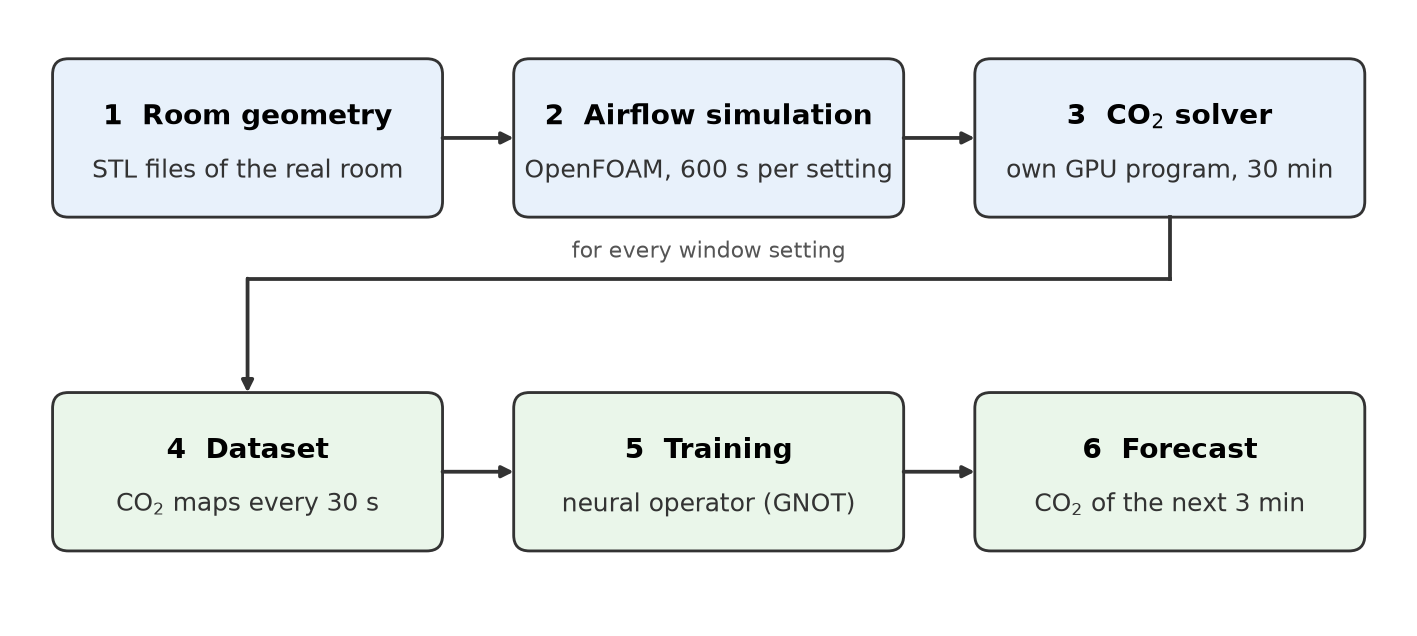
\includegraphics[width=\textwidth]{pipeline.png}
  \caption{Steps from the room to the forecast.}
  \label{fig:pipeline}
\end{figure}

I simulated the room in three steps. In the first setup the windows were opened in three groups and both
doors were open (39 scenarios). In the second setup only the windows W1, W3 and W6 can be opened and door~1 is
open (28 scenarios). Most results in this thesis are from this setup. In the third setup all 8 windows and
both doors can be open or closed. These 40 scenarios are running at the moment. \fref{fig:room} in
\cref{ch:room} shows where the windows and doors are.

\section{What I did}
\begin{itemize}
  \item I reproduced the results of \citet{bian2025} with their code and data.
  \item I built the complete chain from the room geometry to the trained model with open-source software.
  \item I wrote a \cotwo{} solver for the GPU that matches the \cotwo{} of OpenFOAM within about 2\,\%, and I
        found out how often the airflow has to be saved for this.
  \item I built the dataset a second time with this correction and compared the models trained on the old and
        on the new data.
  \item I started the simulations with all windows and doors.
  \item I tested faster simulations, a GPU solver and training without simulation data. These did not become
        part of the final method.
\end{itemize}

\section{Structure}
The thesis follows the order of the work. After the background in \cref{ch:background}, \cref{ch:repro}
shows the reproduction of the paper. \cref{ch:room} is about the room and the OpenFOAM simulations and
\cref{ch:dataset} about the \cotwo{} dataset. The model is described in \cref{ch:model} and its results in
\cref{ch:results}. \cref{ch:sensors} is about the sensor data, \cref{ch:notused} about the things I tested
and did not use, and \cref{ch:conclusion} is the conclusion.
  % Introduction
\chapter{Background}
\label{ch:background}

This chapter explains the ideas that the rest of the thesis builds on: how \cotwo{} behaves in a room, how a
computer can simulate the air in a room, and what a neural operator is.

\section{\cotwo{} in classrooms}
People breathe out air with about 40,000~ppm \cotwo{}, while the outdoor air has about 400~ppm. (The unit ppm
means parts per million, so 40,000~ppm is 4\,\% of the air.) In a closed room the \cotwo{} therefore rises as
long as people are inside, and it can only fall when fresh air comes in. In this thesis, as in
\citet{bian2025}, each person breathes out 6~L/min, so 20 people add about 79~ppm\,m\textsuperscript{3} of
\cotwo{} per second above the outdoor level. For our room of about 450~m\textsuperscript{3} this is roughly
10~ppm more per minute in a closed room, if the air were mixed perfectly (my own calculation).
\todo{guideline values for CO2 in classrooms, e.g. 1000 ppm, with reference}

\section{Airflow simulation}
To know where the \cotwo{} goes, one has to know how the air moves. A computer can calculate this. In
computational fluid dynamics (CFD), the room is cut into many small cells (the mesh), and the program
calculates the air velocity and the pressure in every cell, step by step in time. The equations behind this
are the incompressible Navier--Stokes equations: they say that no air is lost and that the air moves
according to the forces on it, such as pressure differences and friction. (Incompressible means that the
density of the air is treated as constant.)

At the speeds that come through an open window the flow is turbulent: it forms many small, irregular eddies.
The cells of a mesh for a whole room are much larger than the smallest eddies, so these cannot be calculated
directly. In Reynolds-averaged (RANS) models only the average flow is computed, and the effect of the eddies
is described by an additional turbulent viscosity $\nu_t$ (a kind of extra internal friction of the air). I
use the k-$\omega$ SST model of \citet{menter1994}, which is also used by \citet{bian2025} and is common for
indoor airflow. It solves two extra equations, one for the turbulent kinetic energy $k$ (the energy in the
eddies) and one for its specific dissipation rate $\omega$ (how fast this energy is turned into heat), and
computes $\nu_t$ from them. Near walls it behaves like a k-$\omega$ model and in the open room like a
k-$\varepsilon$ model.

The simulations are done with OpenFOAM \citep{weller1998}, a free CFD program, version v2412 from
openfoam.com, with the transient solver \texttt{pimpleFoam}. Even though RANS describes the mean flow, the
transient solution of our room does not become fully steady: the jets from the open windows keep moving, and
the flow fluctuates around a mean pattern (\cref{ch:dataset}).

A different way to simulate the flow is the lattice Boltzmann method \citep{kruger2017}, which is well suited
for GPUs. It is usually combined with a large-eddy simulation (LES), in which the large eddies are resolved
and only the smallest ones are modelled, for example with the model of \citet{smagorinsky1963}. I tested this
idea as a faster alternative in \cref{ch:computation}.

\section{\cotwo{} transport}
The \cotwo{} at a point changes for three reasons: the air carries it along (advection), it spreads out by
itself and through the eddies (diffusion), and the people add new \cotwo{} (source). In an equation:
\begin{equation}
  \frac{\partial c}{\partial t} + \nabla\cdot(\mathbf{u}\,c) = \nabla\cdot\big((D + \nu_t/\mathrm{Sc}_t)\,\nabla c\big) + S,
  \label{eq:co2}
\end{equation}
where $c$ is the \cotwo{} above the outdoor level in ppm, $\mathbf{u}$ the air velocity, $D$ the molecular
diffusivity of \cotwo{} in air, $\mathrm{Sc}_t$ the turbulent Schmidt number and $S$ the source from the
people. The equation is linear in $c$, so the \cotwo{} grows exactly in proportion to the number of people.
Because \cotwo{} does not change the airflow, the flow can be computed first and the \cotwo{} afterwards.

\section{Neural networks and neural operators}
A neural network is a computer program with many adjustable numbers. It learns from examples: it is shown
inputs together with the correct answers, and its numbers are adjusted until its answers come close to the
correct ones (training). After the training it can answer for new inputs, and it does so very fast.

Most networks map a short list of numbers to another list of numbers. Here, the input and the output are not
short lists but whole \cotwo{} maps of the room, with values at thousands of points. A neural operator is a
network built for this: it learns a map between such fields, for example from the \cotwo{} map now to the
\cotwo{} map in three minutes \citep{li2021fno}. GNOT \citep{hao2023gnot} is a neural operator of the
transformer type: the points where an answer is wanted (queries) look at the input data through a mechanism
called attention, which lets each point decide which input values matter most for it. It works on
unstructured point sets, which suits a room with columns and irregular measurement points.

\section{The method of Bian and Shi}
\citet{bian2025} simulated a classroom at UC San Diego with ceiling vents in ANSYS Fluent (k-$\omega$ SST).
They ran 300 simulations of 30~minutes with different vent settings, each starting from a steady state
computed for one of 10 vent settings, and trained a GNOT model that uses the \cotwo{} of the last 6~minutes to
forecast the next 3~minutes, with an uncertainty from a Gaussian likelihood. With an ensemble of five networks
(five networks trained separately, whose forecasts are averaged) they reach a test error of 10.9\,\% in their
metric, and they use the model to choose vent settings that keep the \cotwo{} low with little energy.

\section{Physics-informed learning}
Instead of learning from simulation data, a network can be trained to obey the physical equations
themselves: at many random points of the domain, the network is told how much its answer violates the
equations, and it is adjusted to reduce this \citep{raissi2019}. This idea was also extended to neural
operators \citep{li2021pino}. I tried it for our room in \cref{ch:pinn}.
  % Background
\chapter{Reproducing the paper}
\label{ch:repro}

Before I changed anything, I ran the published code and data of \citet{bian2025} on our lab computer
(NVIDIA RTX A2000, 12~GB). I wanted to see if I get the same accuracy as in the paper.

\section{Setup}
The authors' dataset contains 3,893 training and 1,126 test samples. Each sample holds the \cotwo{}
at 7,492 points of the room for the last 12 time steps (6~minutes), the 13 control values (number of
people and the airflow rate and angle of 6 vent groups) and the \cotwo{} of the next 6 time steps
(3~minutes). The network (GNOT, 552,969 parameters) was trained for 200 epochs, which took about
6~hours per network. I trained five networks with the seeds 2023 to 2027 and used their mean as
the forecast, as in the paper.

\section{Result}
\tref{tab:repro} compares my networks with Table~3 of the paper (relative $\ell_2$ error).

\begin{table}[h]
  \centering
  \caption{My networks compared with the paper.}
  \label{tab:repro}
  \begin{tabular}{lrrrr}
    \toprule
     & \multicolumn{2}{c}{This work} & \multicolumn{2}{c}{Paper}\\
     & Train & Test & Train & Test\\
    \midrule
    Network 1 & 5.85\,\% & 12.70\,\% & 6.35\,\% & 12.09\,\%\\
    Network 2 & 5.88\,\% & 12.71\,\% & 6.33\,\% & 11.83\,\%\\
    Network 3 & 5.84\,\% & 12.70\,\% & 6.33\,\% & 11.82\,\%\\
    Network 4 & 5.92\,\% & 12.53\,\% & 6.35\,\% & 12.74\,\%\\
    Network 5 & 5.81\,\% & 12.97\,\% & 6.33\,\% & 13.01\,\%\\
    Ensemble  & 5.48\,\% & 11.46\,\% & 5.9\,\%  & 10.90\,\%\\
    \bottomrule
  \end{tabular}
\end{table}

The single networks are in the same range as in the paper (12.5--13.0\,\% against 11.8--13.0\,\%),
and the ensemble is clearly better than every single network, as in the paper. My ensemble error is
0.56 percentage points higher than the published one. The values in \tref{tab:repro} use the definition of the
paper, which includes the 400~ppm of the outdoor air. When only the \cotwo{} above the outdoor level counts
(\cref{ch:model}), the same five networks have an error of 29.8\,\% on the test set and 13.8\,\% on the
training set. One difference is the loss: the training
script in the repository trains networks that predict only the mean \cotwo{} with a relative
$\ell_2$ loss, while the paper's networks also predict a variance and are trained with a Gaussian
negative log-likelihood. Different random seeds and hardware may also contribute.

\section{Problems in the published code}
To run the code I had to fix a few things:
\begin{itemize}
  \item the training script called the likelihood loss with the wrong arguments and stopped with
        an error; I used the relative $\ell_2$ loss of the repository instead;
  \item the variant with mean and variance output (GNOTE) failed because a tuple was treated as a
        tensor, and its likelihood loss was never used;
  \item a data file needed by the control notebook had been deleted in a later commit and had to be
        taken from an older commit;
  \item the notebooks expected a second GPU (\texttt{cuda:1});
  \item the code only runs with specific package versions (PyTorch 2.3.0, DGL 2.2.1, NumPy below 2.0).
\end{itemize}
The version with these fixes is in my repository
(\url{https://github.com/Zainhanif700/BuildingControlCFD}). The script \texttt{scripts/run\_evaluation.sh}
runs the evaluation of the five networks.
  % Reproducing the paper
\chapter{The room and the airflow simulations}
\label{ch:room}

\section{The classroom}
The classroom is room 1-130. It is 15.53~m long, 9.16~m wide and 3.15~m high, and the geometry comes from STL
files of the real room. One long wall has 8 windows, which I call W1 to W8. The opposite wall has 2 doors, and
there are 4 round columns in the room (\fref{fig:room}). In the model each window is 0.61~m wide and as high
as the room, and each door is 1.06~m wide and 2.11~m high. Fresh air comes in through the open windows and
goes out through the open doors.

\begin{figure}[h]
  \centering
  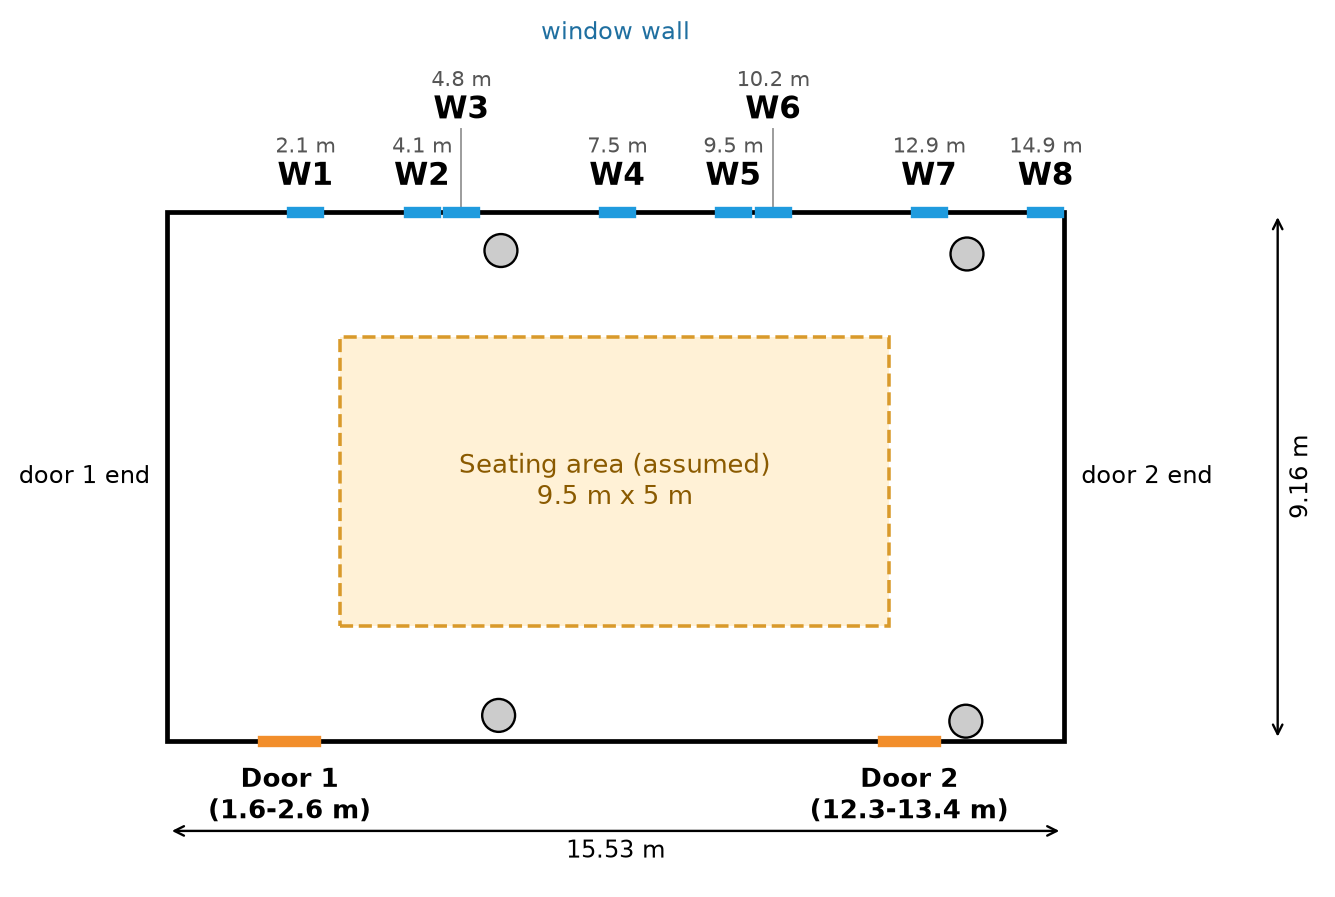
\includegraphics[width=0.95\textwidth]{room_plan.png}
  \caption{Model of classroom 1-130 (top view).}
  \label{fig:room}
\end{figure}

The people sit in a seating area of $9.5\times5$~m in the middle of the room. The \cotwo{} is released there
between 1.0 and 1.2~m height. All simulations use 20 people. Because of \eref{eq:co2} the results can be
scaled to any other number of people.

\section{Window scenarios}
A window scenario says which windows and doors are open and how fast the air comes in through each open
window. I worked with three setups.

In the first setup the 8 windows were opened in three groups (W1--W3, W4--W6, W7--W8) and both doors were
open. I simulated 39 scenarios, 31 for training and 8 for testing.

In the second setup only the windows W1, W3 and W6 can be opened, door~1 is open and door~2 is closed. This
was the plan for the room with the sensors at that time. Each of the three windows is closed or open with an
air speed between 0.2 and 2.0~m/s. I simulated 28 scenarios (\tref{tab:settings}). 8 of the random ones are
only used for testing and the model never sees them in training.

\begin{table}[h]
  \centering
  \caption{The 28 window scenarios of the second setup.}
  \label{tab:settings}
  \begin{tabular}{l>{\raggedright}p{7.6cm}l}
    \toprule
    Scenarios & Windows & Use\\
    \midrule
    N01--N09 & one window open (W1, W3 or W6) at 0.5, 1 or 2~m/s & training\\
    N10--N12 & all three open at 0.5, 1 or 2~m/s & training\\
    N13--N28 & random speeds 0.2--2.0~m/s, each window closed with probability 0.3 & 8 training, 8 test\\
    \bottomrule
  \end{tabular}
\end{table}
The test scenarios are N14, N15, N19, N20, N23, N24, N27 and N28.

In the third setup all 8 windows and both doors can be open or closed (\sref{sec:allopen}).

\section{Simulation setup}
\tref{tab:sim} shows the OpenFOAM settings. At an open window the air comes in with the same speed over the
whole opening. The speed starts at zero and reaches its full value after about 2~s. The open doors are
outlets with a fixed pressure, and air can also come back in through them. Walls, columns, closed windows and
closed doors are walls with wall functions. OpenFOAM also calculates the \cotwo{} itself, and I use this to
check my own \cotwo{} solver (\cref{ch:dataset}).

\begin{table}[h]
  \centering
  \caption{OpenFOAM settings.}
  \label{tab:sim}
  \begin{tabular}{>{\raggedright}p{4.2cm}p{9.5cm}}
    \toprule
    Item & Setting\\
    \midrule
    Solver & OpenFOAM v2412, \texttt{pimpleFoam} (transient), k-$\omega$ SST with wall functions\\
    Mesh & hexahedral, 8~cm cells, 856,284 cells after removing the columns\\
    Air & kinematic viscosity $1.5\times10^{-5}$~m\textsuperscript{2}/s\\
    Inlet & speed $v(t)=v_0\tanh(1.5\,t/\mathrm{s})$, turbulence intensity 5\,\%, length scale 0.1~m\\
    Time step & adaptive, Courant number $\le 1$\\
    Simulated time & 600~s\\
    \cotwo{} source & 20 people, 6~L/min at 40,000~ppm each, spread evenly over the seating area\\
    \cotwo{} in OpenFOAM & $D=1.6\times10^{-5}$~m\textsuperscript{2}/s, $\mathrm{Sc}_t=0.7$\\
    \bottomrule
  \end{tabular}
\end{table}

\section{Simplifications}
The model is simpler than the real room in some points:
\begin{itemize}
  \item In the real room the windows sit 0.15--0.3~m back in the wall. In the model the wall is flat.
  \item The real walls have small steps, and the real ceiling is at 3.13~m instead of 3.15~m.
  \item In the model every window is open over the full height of the room. The real windows are smaller.
        So with real sensor data the measured air speed has to be converted to the same amount of air per
        second before it goes into the model (\cref{ch:sensors}).
  \item When a door is closed, the small gap under it is ignored.
  \item The temperature is not simulated, so warm air does not rise in the model. \citet{bian2025} also assume
        a constant air density and leave out buoyancy, because the air that is pushed in by the ventilation is much
        stronger.
\end{itemize}

\section{Mesh study}
In the very first setup I used a mesh with 10~cm cells. To check if this is good enough for our model, I
simulated two different scenarios with 15, 10 and 8~cm cells and compared the results at 600~s with the 8~cm
mesh (\tref{tab:mesh}). The table below shows the difference of the velocity in the whole room and of the
\cotwo{} at 1.6~m height. I checked the \cotwo{} with two numbers. The first one is the same as in the paper,
which includes the 400~ppm of the outdoor air. The second one uses only the \cotwo{} above the outdoor level,
which is why its error is larger. The last column is the total \cotwo{} in the room divided by the value
of the 8~cm mesh. The 8~cm mesh (856,284 cells) is the reference, so it is not in the table.

\begin{table}[h]
  \centering
  \caption{Mesh study, difference to the 8~cm mesh (856,284 cells).}
  \label{tab:mesh}
  \begin{tabular}{llrrrrr}
    \toprule
    Scenario & Mesh & Cells & Velocity & Paper metric & \cotwo{} at 1.6~m & Total \cotwo{}\\
    \midrule
    S02 & 15~cm & 132,258 & 25.8\,\% & 5.47\,\% & 47.3\,\% & 1.004\\
        & 10~cm & 438,929 & 22.7\,\% & 4.91\,\% & 42.4\,\% & 0.931\\
    S08 & 15~cm & 132,258 & 28.6\,\% & 1.54\,\% & 36.7\,\% & 0.749\\
        & 10~cm & 438,929 & 40.4\,\% & 1.60\,\% & 38.3\,\% & 0.697\\
    \bottomrule
  \end{tabular}
\end{table}

In the faster scenario S08 the 10~cm mesh has about 30\,\% less \cotwo{} in the room than the 8~cm mesh. The
differences do not get smaller from the 15~cm to the 10~cm mesh in S08, and they are still large for the 10~cm mesh
in S02. So this study does not show a mesh-independent solution. I tested these three meshes, and the 8~cm
mesh is the finest of them. I used it for all simulations after the first setup.

I also looked at $y^+$, which tells how well the first cell at the wall fits to the wall functions. On the
8~cm mesh it is between 2 and 140 for S02 and between 21 and 571 for S08, and the mean values are 42 and 163.
The wall functions of OpenFOAM work for small as well as for large values, so I use them without changes.

\section{All windows and doors}
\label{sec:allopen}
In the real room all 8 windows and both doors can be opened, so the second setup with three windows is not
enough. So I simulated a third setup:
\begin{itemize}
  \item each window is closed, or air comes in through it, or air goes out through it;
  \item air comes in with a speed between 0.2 and 2.0~m/s;
  \item each door is open or closed;
  \item in every scenario air comes in through at least one window and can go out through a door or another
        window.
\end{itemize}
There are 40 new scenarios, 10 for each of the four combinations of the two doors. 32 of them are for
training and 8 for testing. Together with the 28 scenarios of the second setup this gives 68 scenarios. The
OpenFOAM settings are the same as before, and the airflow of the first 150~s is saved every second
(\cref{ch:dataset}). The model also gets the information which windows and doors are open.

According to the plan, six windows (W1, W2, W3, W4, W6 and W7) and both doors get a sensor, and the windows
W5 and W8 stay closed. Six of the 40 new scenarios have exactly these two windows closed, and all 28 scenarios
of the second setup fit to this plan as well (with door~2 closed). The results of the model trained on all 68
scenarios are in \cref{ch:results}.
  % The room and the airflow simulations
\chapter{Building the \cotwo{} dataset}
\label{ch:dataset}

\section{Why the \cotwo{} is computed separately}
The forecast model needs the \cotwo{} for 30~minutes per scenario, as in \citet{bian2025}: the \cotwo{} is
still rising after 10~minutes when the ventilation is weak, and 30~minutes give 44 training samples,
because a new sample of 9~minutes (6~minutes of history and 3~minutes of forecast) starts every 30~s. A run of
30~minutes has 61 \cotwo{} maps, one every 30~s, a sample needs 12 maps (6~minutes of history) + 6 maps (3~minutes of forecast) = 18 maps, and so $61 - 18 + 1 = 44$.
A 30-minute OpenFOAM run would take at least
two days per scenario on one core of the computers I work with. I therefore split the work into two parts:
\begin{enumerate}
  \item OpenFOAM computes the airflow for 600~s and saves the velocity and the turbulent viscosity.
  \item My own solver computes the \cotwo{} for the full 30~minutes on the GPU from this airflow. The
        \cotwo{} map is stored every 30~s, which gives the 61 maps of one run.
\end{enumerate}
When the windows open, the airflow needs about 2.5~minutes to develop. After that it fluctuates around the
same pattern, because the window scenario does not change during a run. The \cotwo{} solver therefore uses the
real OpenFOAM flow for the first 150~s. The flow saved between 150 and 600~s is averaged into one mean flow
field, and from 160~s on the solver keeps this mean flow fixed until 30~minutes (the change from the last
real flow to the mean flow takes 10~s). Only the airflow is kept fixed; the \cotwo{} is computed at every
time step.

\section{The \cotwo{} solver}
The solver works on the same 8~cm grid as OpenFOAM and runs on the GPU with PyTorch. It does three things.

First it corrects the airflow from OpenFOAM a little, so that exactly as much air goes out through the open
door as comes in through the windows. Without this correction \cotwo{} would be created or lost in the room.

Then it moves the \cotwo{} with the air. I use an upwind scheme with a limiter, which makes sure that the
\cotwo{} never becomes negative and that the total amount only changes through the people and through the air
that leaves the room. The mixing of the \cotwo{} is $D+\nu_t/\mathrm{Sc}_t$ as in \eref{eq:co2}.

The solver goes forward in small time steps with a Runge--Kutta scheme with three stages. The time step is
chosen so that the air moves at most half a cell in one step. Fresh air comes in with 0~ppm above the outdoor
level, and the \cotwo{} leaves the room with the air through the door.

I checked the solver with five tests (\tref{tab:solvertests}).

\begin{table}[h]
  \centering
  \caption{Tests of the \cotwo{} solver.}
  \label{tab:solvertests}
  \begin{tabular}{>{\raggedright}p{7cm}>{\raggedright\arraybackslash}p{6.7cm}}
    \toprule
    Test & Result\\
    \midrule
    no flow: same result as my first \cotwo{} solver & largest difference 0\\
    flow correction: divergence-free, and the air through the door equals the air through the windows
      & largest relative divergence $1.2\times10^{-11}$; 2.8823 in and 2.8822 out
        (expected 2.8822~m\textsuperscript{3}/s)\\
    uniform \cotwo{} in a closed room with a swirling flow & stays uniform, largest deviation $4.5\times10^{-10}$\\
    closed room with a source & \cotwo{} amount = start amount + added amount (ratio 1.0000)\\
    no negative values (limiter) & smallest value $2.3\times10^{-3}$ in the test case\\
    \bottomrule
  \end{tabular}
\end{table}

My first \cotwo{} solver had no such limiter. In the first dataset it produced small negative values, down
to $-15$~ppm. In one case after 30~minutes, the cells below $-1$~ppm were 1.3\,\% of the cells, and the
negative amount was 0.08\,\% of the total \cotwo{}. In the tests, the new solver does not produce
negative values.

\section{Checks against OpenFOAM}
OpenFOAM computes the \cotwo{} itself on its own flow. I use this as the reference and compare it with my
\cotwo{} at the last OpenFOAM time, in two ways: as the relative $\ell_2$ difference of the \cotwo{} above
the outdoor level in the whole room (strict), and in the metric of \citet{bian2025}, which includes the
400~ppm of the outdoor air and is evaluated on the planes at 1.1 and 1.6~m.

In the first setup the checks showed two weaknesses: the total amount of \cotwo{} was not kept exactly, and
the mean flow mixed the \cotwo{} too little, because the averaging removes the fluctuations. After making the
solver mass-conserving and using a turbulent Schmidt number of $\mathrm{Sc}_t=0.3$ instead of 0.7
\citep{tominaga2007}, the difference in the paper's metric fell from 6--9\,\% to 1--4\,\%. In one scenario
that was simulated in OpenFOAM for the full 30~minutes, my \cotwo{} stayed within about 3\,\% of OpenFOAM's
over the whole time.

I chose the Schmidt number with three scenarios of the first setup (\tref{tab:sct}). The table shows the
difference to the \cotwo{} of OpenFOAM after 10~minutes in the metric of the paper, at 1.1~m and at 1.6~m
height. The values 0.25 and 0.35 are both clearly better than 0.7, so I took 0.3 in the middle.

\begin{table}[h]
  \centering
  \caption{Tests of the Schmidt number.}
  \label{tab:sct}
  \begin{tabular}{lrrr}
    \toprule
    $\mathrm{Sc}_t$ & 3 windows, 1~m/s & 3 windows, 0.5~m/s & 8 windows, 0.5~m/s\\
    \midrule
    0.70 & 7.3 / 6.5\,\% & 6.1 / 5.6\,\% & 2.9 / 2.4\,\%\\
    0.35 & 4.6 / 3.8\,\% & 4.2 / 4.0\,\% & 1.9 / 1.2\,\%\\
    0.25 & 4.0 / 3.0\,\% & 4.2 / 3.8\,\% & 2.7 / 1.4\,\%\\
    \bottomrule
  \end{tabular}
\end{table}

\section{Reproducibility and simulated time}
To check that the data can be reproduced, I simulated scenario N10 a second time
and built its dataset again. The \cotwo{} of both runs differs by 1.1\,\% over all points and times, and by
at most 0.15\,\% in the paper's metric. Using only the first 450~s of the OpenFOAM run instead of 600~s
changes the \cotwo{} by 3.1\,\% (paper's metric at most 0.48\,\%) and would make the simulations about
1.33 times faster.

\section{The save interval of the flow}
Comparing all 28 scenarios with OpenFOAM's \cotwo{} showed large differences in some scenarios with high
window speeds, already when my solver used the real OpenFOAM flow without any averaging (for example
114\,\% in N14 and 131\,\% in N28 after 600~s). The scenarios with these differences all have W1, W3 and W6 open
at speeds between about 0.9 and 2~m/s and a strongly fluctuating flow.

The reason was the save interval. OpenFOAM saved the flow every 10~s, and my solver interpolates linearly
between the saves. At 2~m/s the air moves about 20~m in 10~s, more than the length of the room, so the saves
miss most of what the air does. To test this, I simulated N28 for 150~s with a save every second and computed
the \cotwo{} from every 1st, 2nd, 5th and 10th save (\tref{tab:saves}).

\begin{table}[h]
  \centering
  \caption[Save interval test for N28.]{Save interval test for N28 (difference to OpenFOAM in the whole
  room / total \cotwo{} divided by OpenFOAM's).}
  \label{tab:saves}
  \footnotesize
  \begin{tabular}{lrrrrr}
    \toprule
    Saved every & 30~s & 60~s & 90~s & 120~s & 150~s\\
    \midrule
    1~s  & 3.1\,\% / 1.001 & 2.1\,\% / 0.998 & 2.2\,\% / 0.998 & 2.0\,\% / 1.000 & 2.0\,\% / 1.001\\
    2~s  & 4.3\,\% / 1.004 & 4.4\,\% / 0.999 & 4.0\,\% / 1.002 & 4.0\,\% / 1.008 & 4.7\,\% / 1.012\\
    5~s  & 12.5\,\% / 1.021 & 16.0\,\% / 1.002 & 13.1\,\% / 1.027 & 17.7\,\% / 1.077 & 19.4\,\% / 1.103\\
    10~s & 30.6\,\% / 1.032 & 29.7\,\% / 0.997 & 27.2\,\% / 1.060 & 40.0\,\% / 1.156 & 45.4\,\% / 1.232\\
    \bottomrule
  \end{tabular}
\end{table}

With saves every second my solver matches OpenFOAM within about 2\,\%. N14 gives the same picture: 1.9--3.7\,\%
with 1~s saves and 24--45\,\% with 10~s saves. For the calm scenario N01 (one window at 0.5~m/s) the save
interval hardly matters (25.8\,\% with 10~s and 25.6\,\% with 1~s saves at 150~s, both with $\mathrm{Sc}_t=0.3$).
So my solver itself is accurate; only its input was too coarse in fast scenarios.

\section{The flow after 150~s}
With a run of 450~s and saves every second for N28 and N01, I also tested how the \cotwo{} after 150~s can be
made more accurate (\tref{tab:after150}). The real flow saved every second gives about 2\,\% at all times,
which is the best that is possible with this solver.

\begin{table}[h]
  \centering
  \caption[Methods for the time after 150~s.]{Methods for the time after 150~s (difference to OpenFOAM
  at 450~s, in brackets the paper's metric at 1.1~m).}
  \label{tab:after150}
  \small
  \begin{tabular}{>{\raggedright}p{8.2cm}rr}
    \toprule
    Method & N28 (fast) & N01 (calm)\\
    \midrule
    10~s saves to 150~s, then mean flow, $\mathrm{Sc}_t=0.3$ (first dataset) & 106.9\,\% (3.4\,\%) & 32.8\,\% (10.1\,\%)\\
    1~s saves to 150~s, then mean flow, $\mathrm{Sc}_t=0.3$ & 100.7\,\% (3.2\,\%) & 33.1\,\% (10.2\,\%)\\
    1~s saves to 150~s, then mean flow, $\mathrm{Sc}_t=0.7$ & 143.6\,\% (5.6\,\%) & 35.2\,\% (11.9\,\%)\\
    real flow to 300~s, then the 150--300~s flow in a loop, $\mathrm{Sc}_t=0.7$ & 42.2\,\% (1.5\,\%) & 76.0\,\% (31.6\,\%)\\
    real flow to 450~s (upper limit), $\mathrm{Sc}_t=0.7$ & 1.9\,\% (0.1\,\%) & 1.4\,\% (0.3\,\%)\\
    \bottomrule
  \end{tabular}
\end{table}

Neither alternative works for both scenarios. In the fast scenario the fixed mean flow keeps too much
\cotwo{} in the room (about 1.8 times OpenFOAM's amount in N28 at 450~s): the mean flow has calm zones that trap the
\cotwo{}, while the real, fluctuating flow flushes them. Repeating the real flow in a loop helps there, but in
the calm scenario it is much worse, probably because the slow flow keeps changing and the first part is not
typical for the later part. A turbulent Schmidt number of 0.7 is right while the real flow is used
(1.9\,\% at 150~s instead of 25.6\,\% in N01), but with the mean flow 0.3 is better. I therefore keep the mean
flow after 150~s and treat its error as a known limitation. The only way to remove it would be to simulate
the full 30~minutes in OpenFOAM.

\section{The corrected dataset}
Based on these tests I rebuilt the dataset (data~v3) in the same way for all 28 scenarios:
\begin{itemize}
  \item OpenFOAM is run again for the first 150~s with a save every second;
  \item for 0--150~s my solver uses this flow with $\mathrm{Sc}_t=0.7$, as OpenFOAM;
  \item after 150~s it uses the mean flow of the first dataset with $\mathrm{Sc}_t=0.3$.
\end{itemize}
At 150~s the new dataset matches OpenFOAM's \cotwo{} within 1.0--2.2\,\% in the scenarios I have checked so far (paper's
metric at most 0.1\,\%), compared with up to 45\,\% before.

\tref{tab:v3v2} shows how much the data changed. The differences are in the first minutes, when the fresh air
spreads into the room. After about 10~minutes both datasets become the same, because they use the same mean
flow, and at 30~minutes they are identical. After 20~minutes the corrected and the first dataset differ by at most 0.15\,\%, much less than the accuracy
of my solver. So for 20 of the 28 scenarios I recomputed only the first 20~minutes with the corrected flow and took
the last 10~minutes from the first dataset. This saved GPU time. The other 8 scenarios were recomputed for the full
30~minutes.

\begin{table}[h]
  \centering
  \caption{Difference between the corrected and the first dataset.}
  \label{tab:v3v2}
  \begin{tabular}{lrrrrr}
    \toprule
    Scenario & 1~min & 2.5~min & 5~min & 10~min & 30~min\\
    \midrule
    N01 & 24.8\,\% & 29.3\,\% & 1.4\,\% & 0.2\,\% & 0.0\,\%\\
    N07 & 32.1\,\% & 26.3\,\% & 2.1\,\% & 0.6\,\% & 0.1\,\%\\
    N09 & 34.5\,\% & 18.5\,\% & 1.5\,\% & 0.2\,\% & 0.0\,\%\\
    N10 & 36.8\,\% & 31.1\,\% & 1.8\,\% & 0.4\,\% & 0.1\,\%\\
    N14 & 38.1\,\% & 35.9\,\% & 5.1\,\% & 0.7\,\% & 0.0\,\%\\
    N20 & 29.2\,\% & 23.8\,\% & 0.9\,\% & 0.2\,\% & 0.0\,\%\\
    N27 & 43.8\,\% & 27.2\,\% & 1.9\,\% & 0.4\,\% & 0.0\,\%\\
    N28 & 36.3\,\% & 36.1\,\% & 7.8\,\% & 1.6\,\% & 0.0\,\%\\
    \bottomrule
  \end{tabular}
\end{table}

\section{Paper-like transition data}
In \citet{bian2025} every run starts from the steady state of another scenario. I do the same without new
OpenFOAM runs: for each scenario I start from the \cotwo{} of a randomly chosen other scenario after 30~minutes,
switch off the people, and let the new flow carry this \cotwo{} away. Because \eref{eq:co2} is linear, the
\cotwo{} of the new scenario's people can then be added with any number of people, and the numbers before and
after the change are drawn between 10 and 80 during training, as in the paper.

For the corrected dataset the transition runs had to be computed again for the full 30~minutes. Here the
\cotwo{} only decays, so the difference to the old transition runs does not become small over time.
  % Building the CO2 dataset
\chapter{The forecast model}
\label{ch:model}

\section{Task}
The task is the same as in \citet{bian2025}. The model gets the \cotwo{} maps of the last 6~minutes, which are
12 maps with 30~s between them, and it predicts the \cotwo{} maps of the next 3~minutes, which are 6 maps. I
use the maps at 1.6~m height. On the 8~cm grid this is the cell layer at 1.58~m with 21,956 points. The model
also gets the air speeds of the 8 windows, which windows and doors are open, and the number of people.

\section{Network}
The network is built like GNOT \citep{hao2023gnot}, and \tref{tab:model} shows its settings. The model can be
asked for a prediction at any point of the plane. For each of these points it knows the position and the
\cotwo{} history at this point. To know what happens in the rest of the room, it also gets the \cotwo{} history
at 900 fixed points that are spread over the plane, together with the window speeds and the number of people.
In three attention blocks each point collects the information it needs from these inputs.

The network does not predict the \cotwo{} value directly. It predicts how much the \cotwo{} changes compared
with the last known value, for each of the 6 future times. It also predicts a variance, so the model says how
sure it is.

\begin{table}[h]
  \centering
  \caption{The forecast model.}
  \label{tab:model}
  \begin{tabular}{>{\raggedright}p{4cm}p{9.7cm}}
    \toprule
    Item & Value\\
    \midrule
    Input & \cotwo{} of the last 6~min on the 1.6~m plane (12 maps), 8 window speeds, which windows and doors are open, number of people\\
    Output & \cotwo{} change for the next 3~min (6 maps) with variance\\
    Network & cross-attention blocks (GNOT type), 3 blocks, width 128, 4 heads, about 480,000 parameters\\
    Loss & Gaussian negative log-likelihood, as in the paper\\
    Optimiser & AdamW, learning rate $5\times10^{-4}$ with one-cycle schedule, 20,000 steps,
               8 samples $\times$ 1,024 points per step\\
    Ensemble & 5 networks with different random seeds, the forecast is their mean\\
    Hardware, time & NVIDIA RTX A2000 (12~GB), about 1.5~h for the 5 networks\\
    \bottomrule
  \end{tabular}
\end{table}

\section{Training data}
One training sample is 9~minutes long. It has 6~minutes of history and the 3~minutes that the model should
predict. A run of 30~minutes has 61 \cotwo{} maps, one every 30~s. A sample needs 12 maps (6~minutes of history) and 6 maps
(3~minutes to predict), which are 18 maps, and a new sample starts at every map. So a run gives $61 - 18 + 1 = 44$ such
samples. I use two kinds of runs:
\begin{itemize}
  \item In a \emph{direct run} the room starts with fresh air and the \cotwo{} of the people builds up.
  \item In a \emph{transition run} the room starts with the \cotwo{} that was left from another window
        scenario (\cref{ch:dataset}). This is how the runs in the paper start. The number of people before and
        after the change is chosen randomly between 10 and 80.
\end{itemize}
The transition runs have one limit. The airflow of the new scenario starts from still air and not from the
moving air of the scenario before. Also the windows never change during the 6~minutes of history, so the
model has not seen this case in training.

\section{Error measures}
\subsection*{The relative error}
For one sample I calculate the relative $\ell_2$ error of the forecast over all points of the plane and the
6 future times, as in equation~12 of \citet{bian2025}:
\begin{equation}
  e = \frac{\|\hat{c} - c\|_2}{\|c\|_2},
\end{equation}
where $\hat{c}$ is the forecast and $c$ is the simulated \cotwo{}. The error I report is the mean of $e$ over all
test samples.

\subsection*{Two definitions of the \cotwo{}}
The value of $c$ can be defined in two ways. In the definition of the paper, $c$ is the total \cotwo{} in ppm,
including the 400~ppm of the outdoor air. I checked this in the data of the paper: the values to forecast lie
between 396 and 1,109~ppm. The second definition counts only the \cotwo{} above the outdoor level, so $c$ is
the total value minus 400~ppm. The 400~ppm are always there and nobody has to forecast them, so the second
definition is stricter and shows better what the model has learned.

Both definitions use the same mistake in ppm, but they divide it by a different number. An example: the
\cotwo{} will be 610~ppm, and the model says 609~ppm. The mistake is 1~ppm. In the definition of the paper
the error is $1/610 = 0.16\,\%$, and above the outdoor level it is $1/210 = 0.5\,\%$. So the paper's definition
gives smaller percentages for every model. For my reproduction of the paper the two definitions give 11.46\,\%
and 29.8\,\% (\cref{ch:repro}).

I use the definition of the paper to compare with the paper, and I give the stricter value next to it. The text
always says which definition a number belongs to.

\subsection*{Persistence}
An error value alone does not tell if a model is good. So I compare the model with the simplest forecast, that
the \cotwo{} in 3~minutes is the same as now. I call this persistence. The error of persistence also shows how
much the \cotwo{} changes in 3~minutes. A useful model has to be clearly better than persistence. Our open
windows change the air in the room much faster than the ceiling vents in the paper, so the error values of the
paper and mine cannot be compared directly. The comparison with persistence on the same data is the fairest
one.

\subsection*{Test scenarios}
The test scenarios are complete scenarios that the model has never seen in training, so every window setting in
the test is new for the model. This is harder than testing on other time windows of scenarios that were used in
training. The first split has 52 training and 16 test scenarios (8 of the second setup and 8 of the new ones).
Because one split can be lucky or unlucky, I repeated the tests for the sensor model on three other random
splits with 8 and 8 test scenarios.

\subsection*{Room average and warning}
For the use in the room I also report two numbers that are easier to understand than a percentage. The first is
the error of the average \cotwo{} in the seating area in ppm. It is the mean absolute difference between the
forecast and the simulation, taken over the 6 future times. The second is a warning test. The model warns if its
forecast for the next 3~minutes reaches a limit (700 or 800~ppm), minus a safety margin. A real case is a time
when the average \cotwo{} in the seating area really passes the limit within the next 3~minutes. A case is
\emph{found} if the model warned, \emph{missed} if it did not, and a warning without a real case is a
\emph{false alarm}.

\subsection*{What the errors mean}
All errors in this thesis are measured against my simulated data. They show how well the model has learned the
simulation. They do not show how close the simulation is to the real room, because I have no measurements from
the room with the new sensors yet. I chose some settings of the sensor model on the first split, so I use the
random splits as the fairer numbers.
  % The forecast model
\chapter{Results}
\label{ch:results}

\section{First setup}
In the first setup the windows were opened in three groups, both doors were open and the mesh had 10~cm
cells. I trained the model on the transition runs of 31 scenarios and tested it on the other 8. The test error
is 0.11\,\% of the \cotwo{} above the outdoor level. Persistence has 0.39\,\%, so the model is about 4 times
better. In the paper's metric the values are 0.01\,\% and 0.05\,\%. I also trained the model with only 5, 10
and 20 of the training scenarios. \fref{fig:lc1} shows that the error goes down fast at the beginning and
changes only a little between 20 and 31 scenarios.

\fref{fig:s37series} and \fref{fig:s37maps} show one test scenario of the first setup. In S37 only the windows
W7 and W8 are open, and the model did not see this scenario in training. The lines are the simulation and the
dots are the forecasts of the model, each made 3~minutes before. In the first minutes the \cotwo{} of the
scenario before is pushed out of the room, and after that the \cotwo{} of the people builds up slowly. The
maps show that the forecast and the simulation look the same, and the difference is only a few ppm.

\begin{figure}[h]
  \centering
  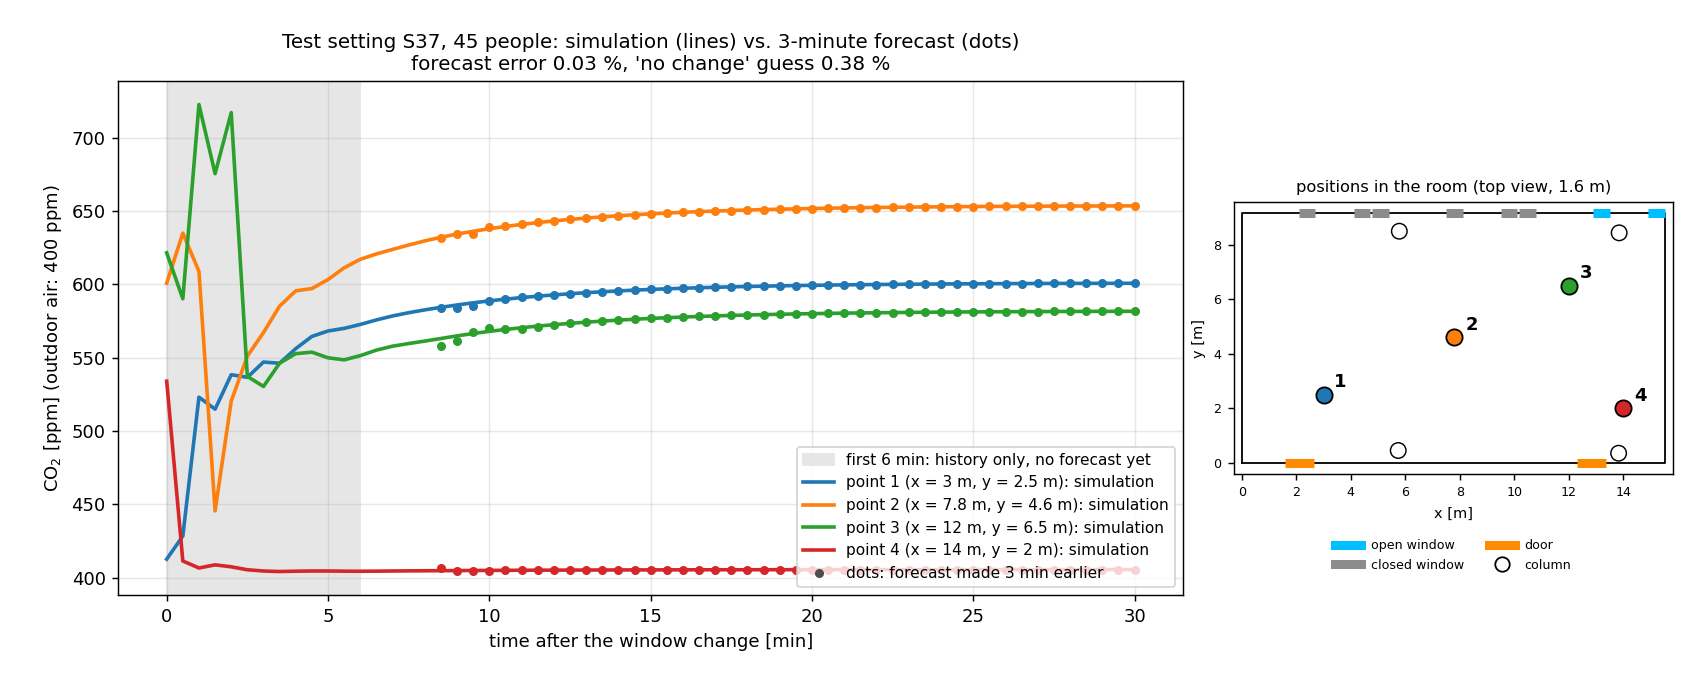
\includegraphics[width=\textwidth]{s37_series.png}
  \caption{Test scenario S37, \cotwo{} at four points.}
  \label{fig:s37series}
\end{figure}

\begin{figure}[h]
  \centering
  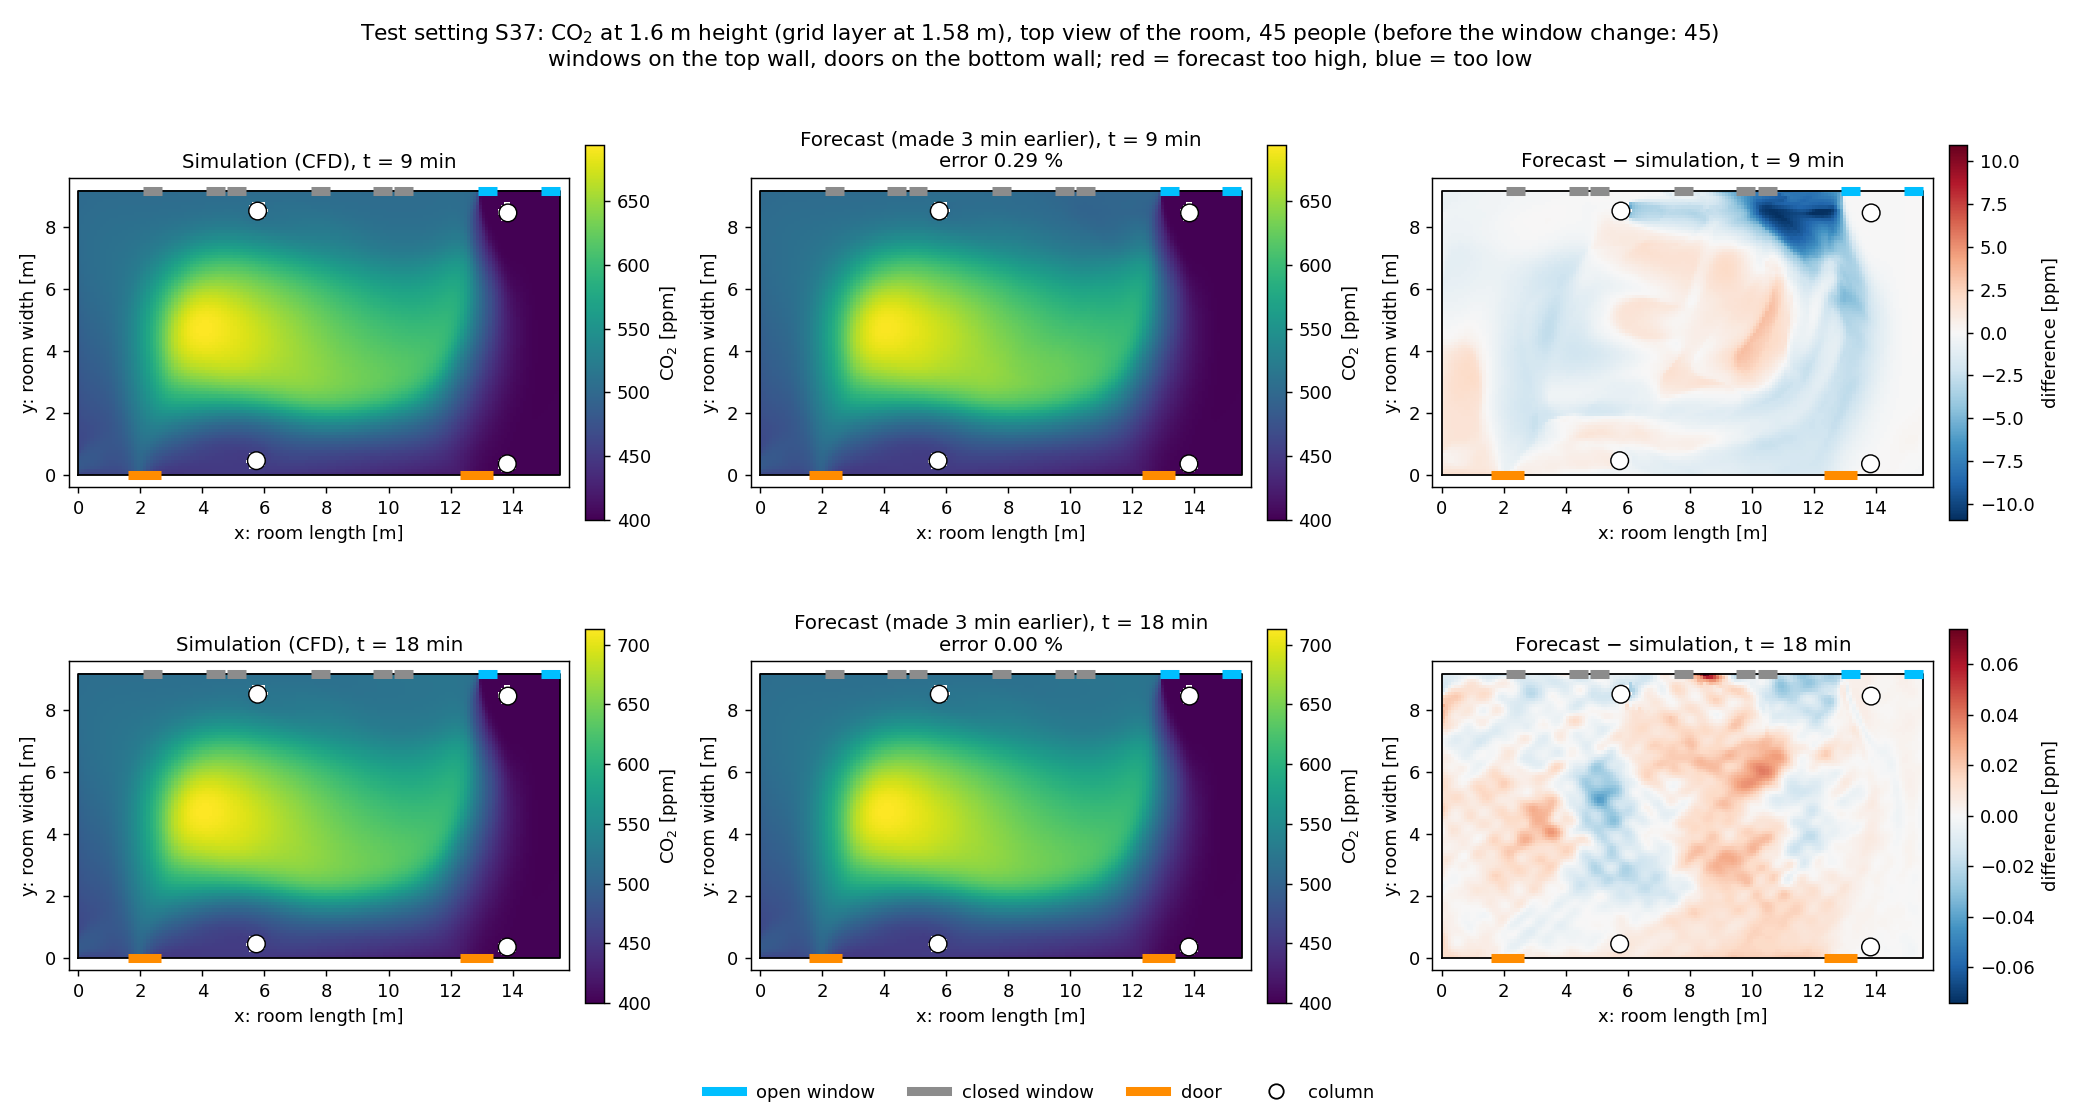
\includegraphics[width=\textwidth]{s37_maps.png}
  \caption{Test scenario S37, simulation and forecast.}
  \label{fig:s37maps}
\end{figure}

\begin{figure}[h]
  \centering
  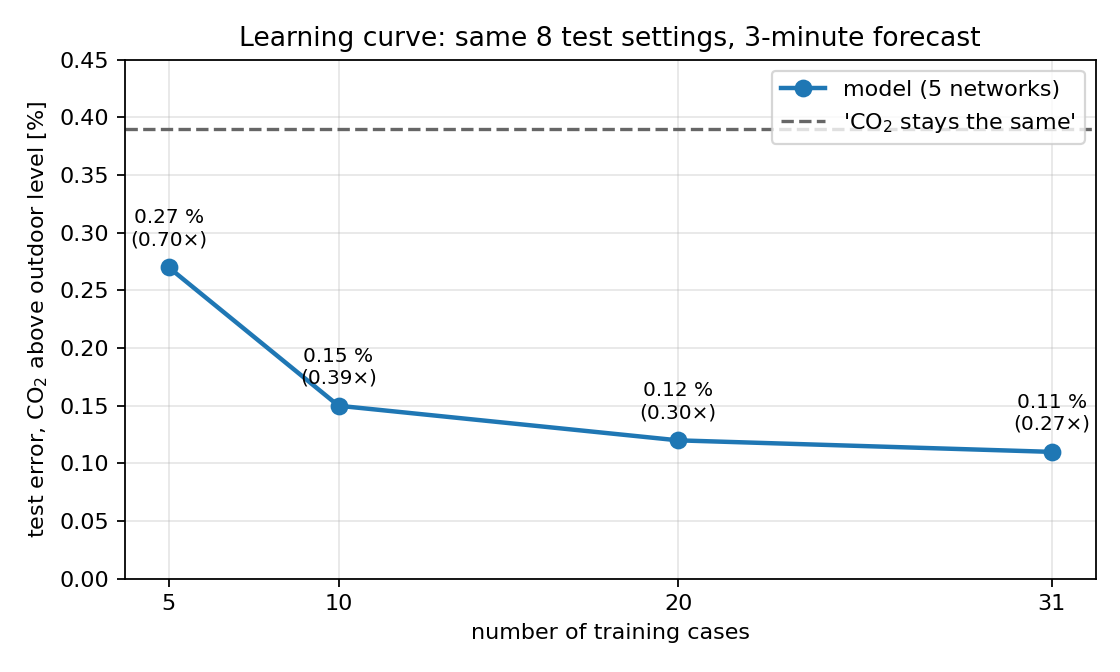
\includegraphics[width=0.75\textwidth]{learning_curve.png}
  \caption{Learning curve of the first setup.}
  \label{fig:lc1}
\end{figure}

\section{Second setup}
In the second setup the windows W1, W3 and W6 can be opened, and the mesh has 8~cm cells. There are 20
scenarios for training and 8 for testing. With the first dataset and the transition runs the test error is
0.61\,\% and persistence has 2.74\,\%, so the model is 4.5 times better. \tref{tab:lc} shows the test error
for fewer training scenarios. With 15 scenarios the result is almost the same as with 20.

\begin{table}[h]
  \centering
  \caption{Learning curve of the second setup.}
  \label{tab:lc}
  \begin{tabular}{lrrrr}
    \toprule
    Training scenarios & 5 & 10 & 15 & 20\\
    \midrule
    Test error & 0.76\,\% & 0.71\,\% & 0.62\,\% & 0.61\,\%\\
    \bottomrule
  \end{tabular}
\end{table}

\section{First and corrected dataset}
In \cref{ch:dataset} I built the dataset of the second setup again with the airflow saved every second. To
see what this means for the forecast, I trained the model two times in exactly the same way. Model A is
trained on the first dataset and model B on the corrected dataset. Then I tested both models on the test
scenarios of both datasets.

\tref{tab:ab} shows the result for the direct runs. On the corrected data model B has an error of 0.33\,\%
and model A 0.37\,\%. Both are about 10 times better than persistence. On the first data both models are
equally good.

\begin{table}[h]
  \centering
  \caption[Models A and B, direct runs.]{Test error of models A and B for the direct runs (in brackets the
  paper's metric).}
  \label{tab:ab}
  \begin{tabular}{lrr}
    \toprule
     & Tested on first data & Tested on corrected data\\
    \midrule
    Model A (trained on first data) & 0.30\,\% (0.043\,\%) & 0.37\,\% (0.049\,\%)\\
    Model B (trained on corrected data) & 0.30\,\% (0.044\,\%) & 0.33\,\% (0.046\,\%)\\
    Persistence & 3.15\,\% (0.420\,\%) & 3.20\,\% (0.421\,\%)\\
    \bottomrule
  \end{tabular}
\end{table}

\tref{tab:ab_cases} shows the error for each test scenario. Model B is better in the scenarios with high
window speeds (N14, N27, N28). These are the scenarios where the data changed most. In the calm scenarios both
models are the same.

\begin{table}[h]
  \centering
  \caption[Test error per test scenario.]{Test error per test scenario on the corrected data in \%
  (direct runs).}
  \label{tab:ab_cases}
  \footnotesize
  \begin{tabular}{lrrrrrrrr}
    \toprule
     & N14 & N15 & N19 & N20 & N23 & N24 & N27 & N28\\
    \midrule
    Model A & 0.23 & 0.58 & 0.12 & 0.08 & 0.25 & 1.17 & 0.23 & 0.32\\
    Model B & 0.14 & 0.59 & 0.09 & 0.08 & 0.23 & 1.16 & 0.16 & 0.21\\
    Persistence & 1.32 & 5.62 & 2.58 & 1.43 & 3.29 & 7.24 & 1.90 & 2.25\\
    \bottomrule
  \end{tabular}
\end{table}

I did the same comparison with the transition runs (\tref{tab:abtr}). Here the difference between the two
models is smaller. On the corrected data model B has 0.64\,\% and model A 0.67\,\%, and persistence has
2.57\,\%. Model A on the first data gives 0.61\,\% again, the same value as in the section before.

\begin{table}[h]
  \centering
  \caption[Models A and B, transition runs.]{Test error of models A and B for the transition runs (in
  brackets the paper's metric).}
  \label{tab:abtr}
  \begin{tabular}{lrr}
    \toprule
     & Tested on first data & Tested on corrected data\\
    \midrule
    Model A (trained on first data) & 0.61\,\% (0.240\,\%) & 0.67\,\% (0.247\,\%)\\
    Model B (trained on corrected data) & 0.60\,\% (0.235\,\%) & 0.64\,\% (0.239\,\%)\\
    Persistence & 2.74\,\% & 2.57\,\%\\
    \bottomrule
  \end{tabular}
\end{table}

Each model was trained only one time with 5 networks, so a part of the difference can be chance. But the
difference shows up in the scenarios with high window speeds and not in the others, which fits to the
correction of the data. For the next trainings I use the corrected dataset.

\section{All windows and doors}
The 40 new scenarios with all windows and doors (\sref{sec:allopen}) are running at the moment. When they are
finished, I will train the model on all 68 scenarios. The model then also gets the information which windows
and doors are open. I will compare it with the results of the second setup and look at how many scenarios are
needed.
  % Results
\chapter{Towards real sensor data}
\label{ch:sensors}

\section{The sensor network}
A wireless sensor network (WSN) is being installed in classroom 1-130. The sensors are built into stations,
and one station is placed next to a window or a door. \tref{tab:station} shows what one station measures. The
air speed sensor gives only the speed and not the direction of the air. The distance sensor is used to see if
the window or door is open or closed. A station can send its values every 30~s, which is the same time step
as in my model.

\begin{table}[h]
  \centering
  \caption{Sensors of one station.}
  \label{tab:station}
  \begin{tabular}{lll}
    \toprule
    Sensor & Measures & Used for\\
    \midrule
    SCD41 & \cotwo{}, temperature, humidity & \cotwo{} history of the model\\
    PAV1015V & air speed & window speed\\
    VL53L1X & distance & window or door open or closed\\
    \bottomrule
  \end{tabular}
\end{table}

According to the plan, six of the eight windows (W1, W2, W3, W4, W6 and W7) and both doors get a station,
so there are eight stations, and all of them measure \cotwo{}, temperature and humidity. The windows W5 and W8
stay closed. \fref{fig:stations} shows where I assume the stations for now. Each station stands in front of its
window or door and points at it. The stations send their values to a server, which stores them in a database
together with the position of each station in the room.

A \cotwo{} sensor already stands in the middle of the room, right next to the projector, and it is running. It
is an older station and belongs to another system, but its data can be read in the same way. The exact position
and height are not known yet.

\begin{figure}[h]
  \centering
  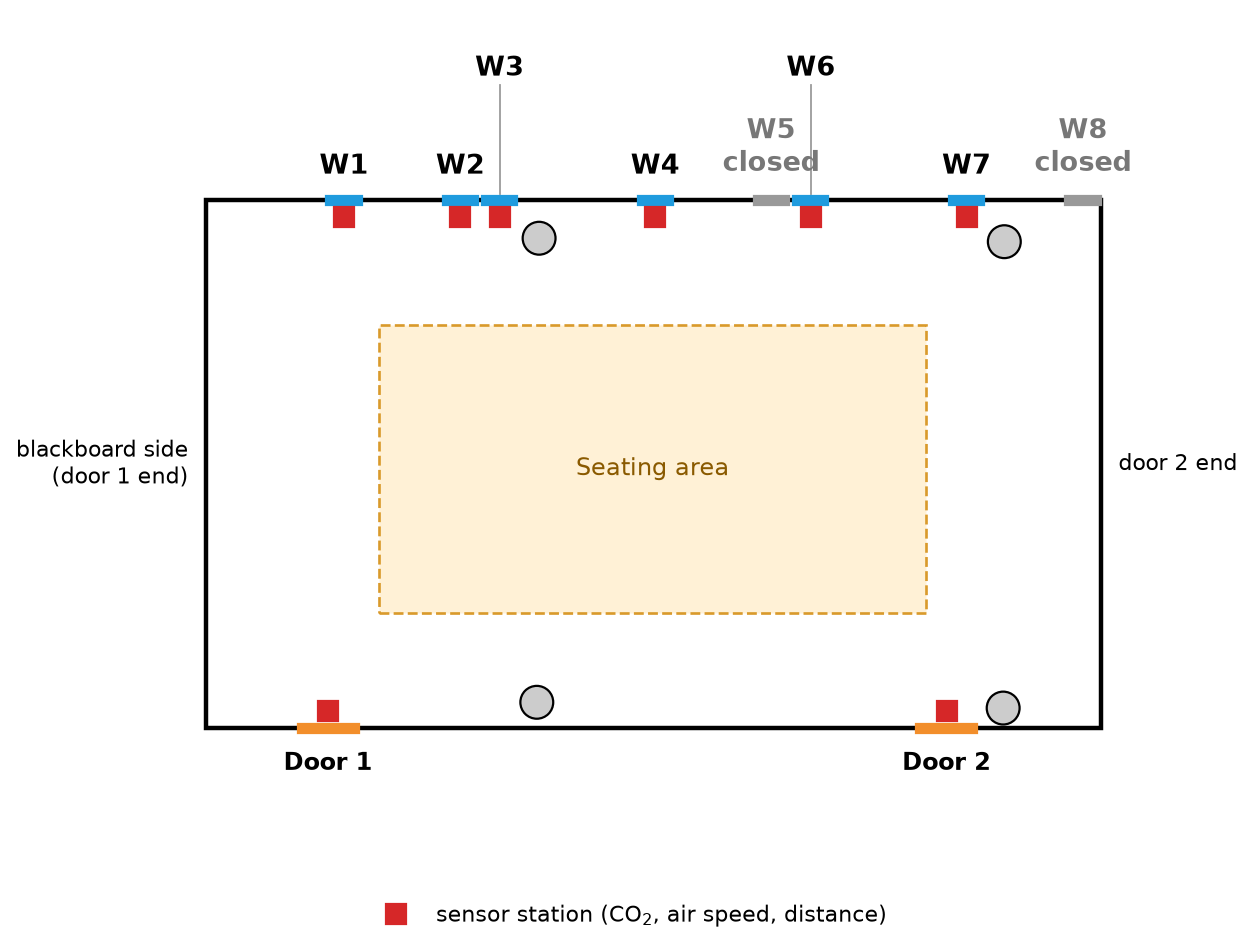
\includegraphics[width=0.9\textwidth]{sensor_stations.png}
  \caption{Sensor stations in classroom 1-130.}
  \label{fig:stations}
\end{figure}

\section{Data flow}
The model was trained on simulated \cotwo{} maps. To use it with the real sensors, the data has to go through
these steps:
\begin{enumerate}
  \item The stations measure the \cotwo{}, the air speed and the distance and send them to the server.
  \item A reader gets the values from the server, from the database or from an exported file.
  \item A mapper brings the values into the form of the model. It puts them on the 30~s time steps, decides
        from the distance if a window is open, assigns each station to its window or door and converts the
        measured air speed into the window speed of the model.
  \item The model predicts the \cotwo{} of the next 3~minutes.
  \item The forecast is shown or used to decide about the windows.
\end{enumerate}
The reader and the mapper are separate, so the rest does not change if the data comes from a file first and
from the database later.

\section{Differences between the sensors and the model}
\begin{itemize}
  \item The model of \cref{ch:model} uses the \cotwo{} history at 900 points of a plane. The sensors give only
        eight points near the windows and doors. The network can work with any set of points, so I trained a
        second model, the \emph{sensor model}, which only gets the history at the station positions. It still
        has to forecast the \cotwo{} for the whole room.
  \item The sensor measures the air speed at one place of a window. The model needs the amount of air that
        comes in through the whole opening. In winter the windows are only tilted, so the opening is much
        smaller than in the simulations. The measured speed has to be converted.
  \item The air speed sensor does not show if air comes in or goes out through a window.
  \item The number of people is not measured yet.
  \item Temperature and humidity are measured, but the model does not use them.
\end{itemize}
I checked these points in \cref{sec:sensorchecks}.

\section{Synthetic sensor data}
Until the real stations deliver data, I produce sensor data from my simulations. I take the \cotwo{} at the
positions of the stations every 30~s and add noise of 10~ppm, as a real \cotwo{} sensor has. I add the window
speeds, the open and closed states and the number of people in the same format as the real data, with the
values multiplied by $10^6$ as on the server. With this data the whole chain from the stations to the forecast
can be tested before the real data comes.

To get a time series like a real lecture, I build the \cotwo{} for a changing number of people. \cotwo{} is
carried by the air without changing it, and the flow in a scenario does not change. Then the \cotwo{} for a
changing number of people is the simulated response to a constant number of people, shifted in time and added
up for every change. For the lecture below I assumed 5 people at the start, 25 after 5~minutes, 45 after
10~minutes and 25 after 25~minutes, and a starting level of 420~ppm.

\section{Test setup}
The sensor model was trained on the 52 training scenarios and tested on 16 scenarios it had never seen. Because
this split can be lucky or unlucky, I repeated the tests on three other random splits of the 68 scenarios. I
report the error as in \cref{ch:model}, in the definition of the paper, which adds the 400~ppm of the outdoor air.
Because this makes all errors look small, I add two numbers that are easier to understand:
\begin{itemize}
  \item the error of the average \cotwo{} in the seating area in ppm, and
  \item a warning test. The model warns if its forecast for the next 3~minutes reaches a limit minus a safety
        margin. I count how many of the real cases, where the \cotwo{} in the seating area passes the limit
        within 3~minutes, the model finds, and how many false alarms it gives.
\end{itemize}
As reference I use persistence, which says that the \cotwo{} stays as it is now. Persistence uses the true
\cotwo{} map of now, which the sensors do not have, so it is only a reference.

\section{Results with the eight stations}
With the eight real stations the error is about 5 to 6\,\% in the definition of the paper (5.3 to 6.5\,\% on the
three random splits). The error of the average \cotwo{} in the seating area is about 20 to 26~ppm, where the
average level is about 520~ppm. In the stricter measure of \cref{ch:model}, which counts only the \cotwo{} above
the outdoor level, the error over the plane at 1.6~m is about 32\,\% on the three random splits (44\,\% on the first
split). For the model of the paper, which I reproduced, the same measure gives 29.8\,\% (\cref{ch:repro}). The sensor
model is much worse than the model with the full map (0.46\,\%), because the stations stand at the walls, where the
air is mostly fresh, and they hardly see the middle of the room, where the people sit.

\tref{tab:compare} puts the numbers next to each other. Both definitions are shown, because the 400~ppm of outdoor
air makes the errors in the definition of the paper much smaller. In the strict definition the paper does not give
a value. For my reproduction of the paper I calculated 29.8\,\%, and my sensor model has about 32\,\%, so the two
values are close. The difference is not large, although the sensor model sees only eight stations and the
reproduced model sees 7,492 points of the room. The two problems are different, so I use this only for orientation
and not as a direct comparison.

\begin{table}[h]
  \centering
  \caption[Comparison with the paper.]{Errors for the next 3~minutes on the test data.}
  \label{tab:compare}
  \small
  \begin{tabular}{lrr}
    \toprule
    Model & Definition of the paper & Strict (above the outdoor level)\\
    \midrule
    Paper (Bian et al.) & 10.9\,\% & not given\\
    My reproduction of the paper & 11.46\,\% & 29.8\,\%\\
    Sensor model, eight stations & about 5 to 6\,\% & about 32\,\%\\
    Main model with the whole map & 0.16\,\% & 0.46\,\%\\
    \bottomrule
  \end{tabular}
\end{table}

I also tried to improve the sensor model. I used a longer history (12 and 20~minutes), spread the station values
over the whole room, changed the loss, used smaller networks, added more noise and gave the model physical
numbers such as the fresh-air flow. This gave no clear gain, at best about one percentage point. Training with
more scenarios did not help either. The numbers of these tests are in Appendix~\ref{app:sensortests}.

\section{A sensor in the middle of the room}
To test this, I added virtual sensors in the seating area to the simulation. \tref{tab:virtual} shows the result.

\begin{table}[h]
  \centering
  \caption[Virtual sensors in the seating area.]{Virtual sensors in the seating area (simulation only), on the
  16 test scenarios of the first split. The warning column gives the cases found out of 15 where the \cotwo{}
  passes 700~ppm.}
  \label{tab:virtual}
  \small
  \begin{tabular}{p{4.6cm}>{\raggedleft\arraybackslash}p{2.6cm}>{\raggedleft\arraybackslash}p{2.9cm}>{\raggedleft\arraybackslash}p{2.2cm}}
    \toprule
    Setup & Error, definition of the paper & Seating-area error [ppm] & Warning found\\
    \midrule
    Eight stations & 6.3\,\% & 26.5 & 13 of 15\\
    Plus one sensor in the middle & 5.0\,\% & 11.4 & 14 of 15\\
    Plus a grid of 16 sensors & 3.6\,\% & 3.5 & 14 of 15\\
    Persistence (true map) & 0.5\,\% & 2.0 & 14 of 15\\
    \bottomrule
  \end{tabular}
\end{table}

One sensor in the middle lowers the error of the room average from 26.5 to 11.4~ppm. The exact place hardly
matters: the middle, the door side, the window side and the back of the seating area gave about the same
result. Only one place on the blackboard side gave no gain, and I do not know why. A projector hangs in the
middle or the back of the room, so the sensor next to it should help. The virtual sensors read the exact
simulated \cotwo{} plus noise, so a real sensor can be less clean.

\section{Warning}
\tref{tab:warning} shows the warning test on three random splits (58 real cases at 700~ppm and 33 at 800~ppm).
Without a margin the model finds 71\,\% of the cases at 700~ppm and 70\,\% at 800~ppm. With a margin of 50~ppm it
finds 91\,\% and 88\,\%, with more false alarms. The margin should not be chosen on the data it is tested on.
When I chose it on two splits and counted on the third, the model found 88\,\% at 700~ppm and 79\,\% at 800~ppm.
The best margin differs between the splits, so it has to be checked with real data.

\begin{table}[h]
  \centering
  \caption[Warning test.]{Warning test on three random splits, simulation only.}
  \label{tab:warning}
  \small
  \begin{tabular}{p{6.2cm}>{\raggedleft\arraybackslash}p{2.3cm}>{\raggedleft\arraybackslash}p{1.6cm}>{\raggedleft\arraybackslash}p{2.2cm}}
    \toprule
    Rule & Cases found & Missed & False alarms\\
    \midrule
    700~ppm, no margin & 41 of 58 & 17 & 9\\
    700~ppm, margin 50~ppm & 53 of 58 & 5 & 32\\
    800~ppm, no margin & 23 of 33 & 10 & 0\\
    800~ppm, margin 50~ppm & 29 of 33 & 4 & 3\\
    700~ppm, margin chosen on the other splits & 51 of 58 & 7 & 25\\
    800~ppm, margin chosen on the other splits & 26 of 33 & 7 & 8\\
    \bottomrule
  \end{tabular}
\end{table}

In the real room, W5 and W8 stay closed. Many of my hard test scenarios open these windows. On the test
scenarios in which they are closed, the error is about 5\,\% in the definition of the paper, and with a margin of 50~ppm
the warning finds 92\,\% of the cases at 700~ppm and 87\,\% at 800~ppm. These scenarios are mostly the simpler
ones with only W1, W3 and W6 open, so this result is easier.

\fref{fig:lecture24} shows the synthetic lecture described above for scenario N24. The warning for 700~ppm
starts 3.5~minutes before the \cotwo{} passes this level, and the model found all 24 time steps with a real case,
with one false alarm. The warning for 800~ppm comes although the \cotwo{} stays below it (the peak is
769~ppm). This is the effect of the safety margin: the model warns from a forecast of 750~ppm, and the real peak
is close to it. The forecast is too low while the students arrive and too high after some leave, because the
model does not know the number of people. \fref{fig:lecture23} shows a quieter lecture in scenario N23, where the
\cotwo{} stays below 700~ppm and the model gives no warning.

\begin{figure}[h]
  \centering
  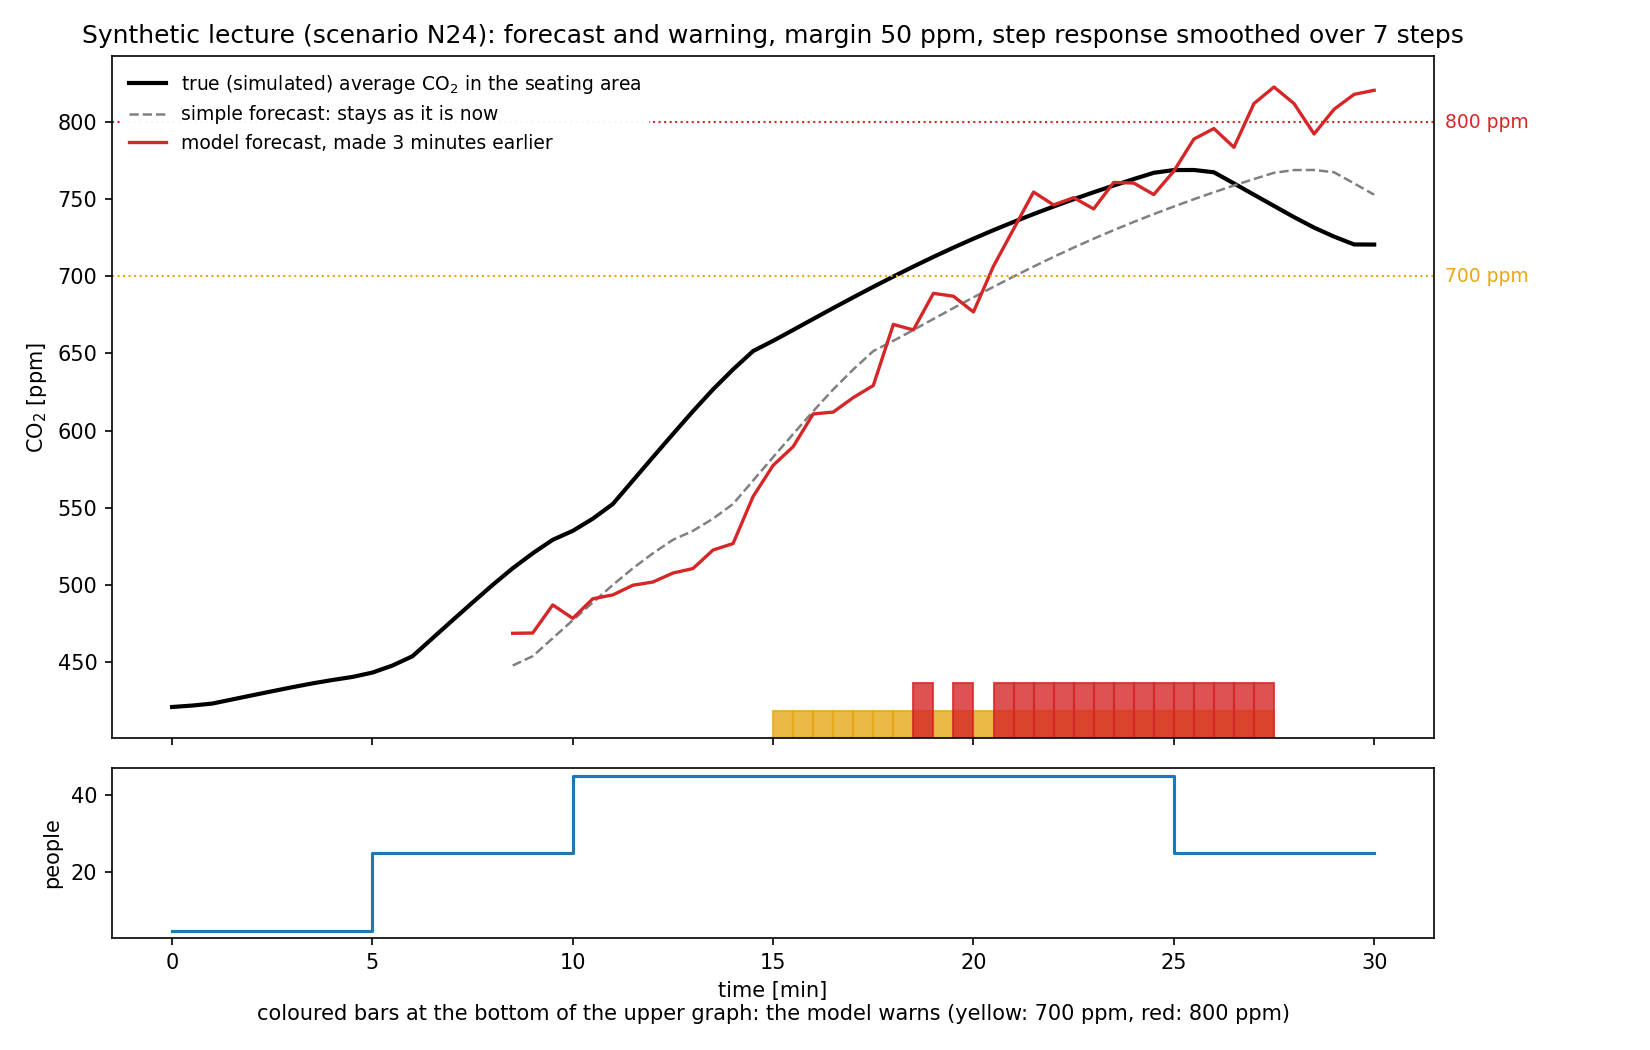
\includegraphics[width=\textwidth]{lecture_N24.png}
  \caption[Synthetic lecture, scenario N24.]{Synthetic lecture in scenario N24 (simulation). Black: true average \cotwo{}
  in the seating area. Red: forecast made 3~minutes earlier. Grey: the forecast that the \cotwo{} stays as it is now.
  The bars at the bottom show when the model warns (yellow: 700~ppm, red: 800~ppm). The number of people (5, 25, 45,
  then 25) is my assumption. The step response of the simulation is smoothed.}
  \label{fig:lecture24}
\end{figure}

\begin{figure}[h]
  \centering
  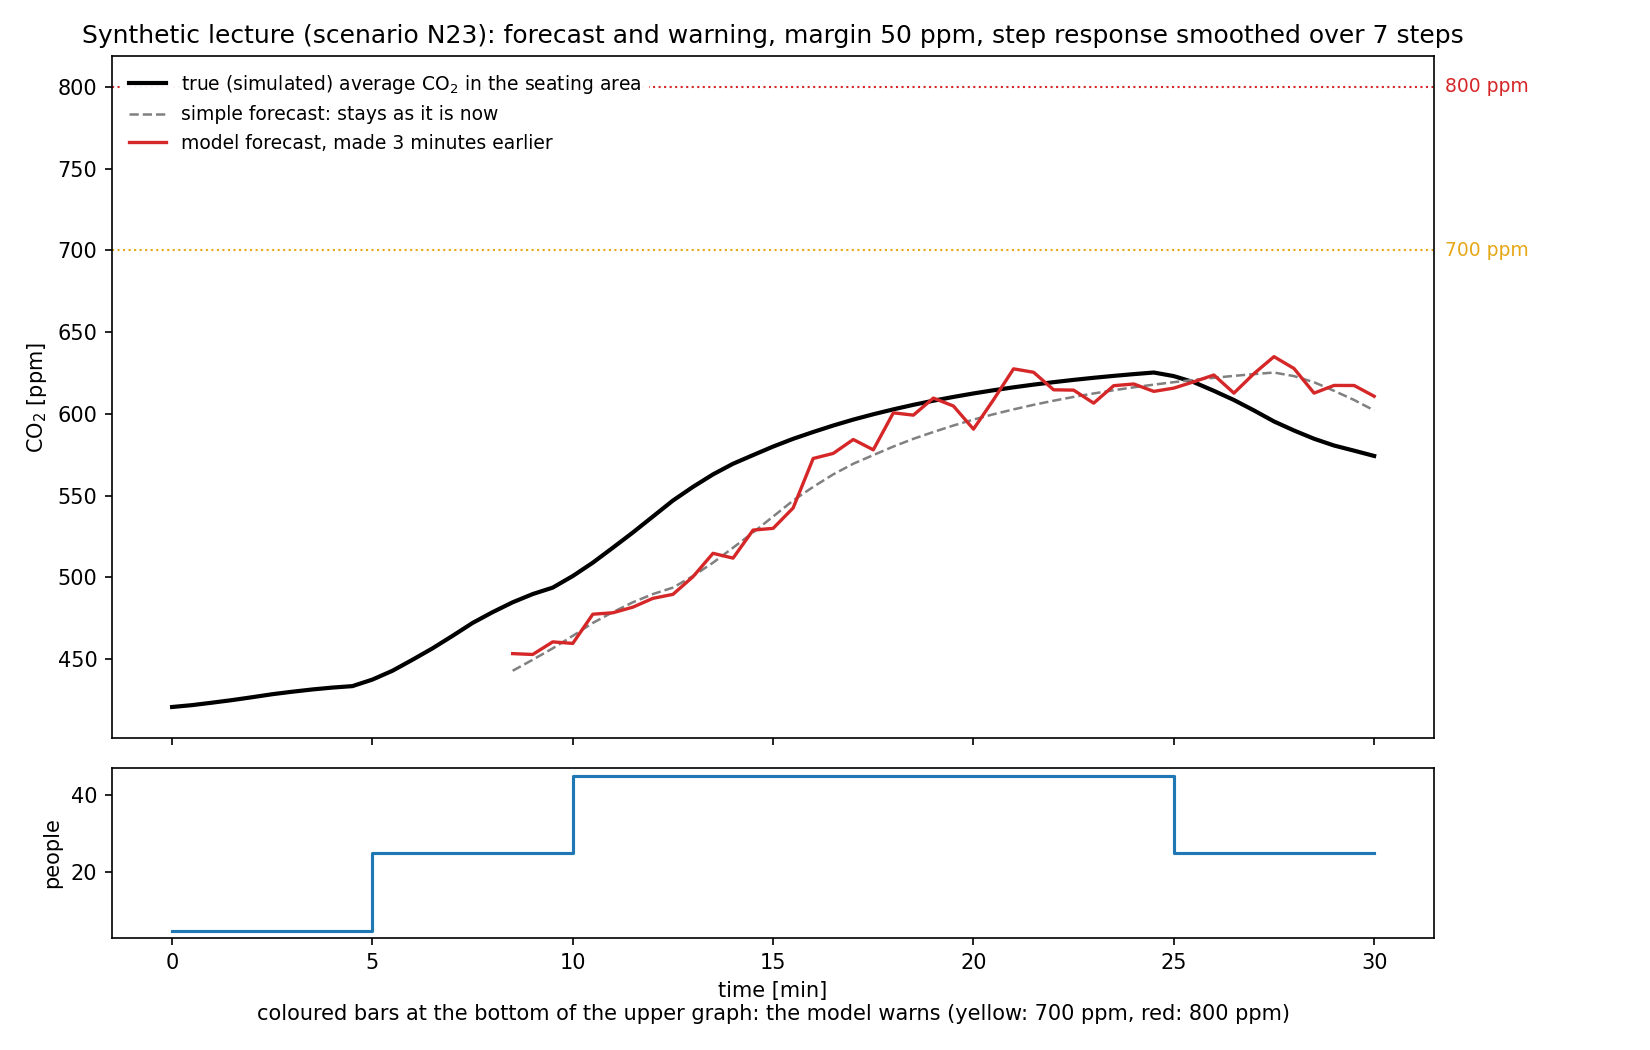
\includegraphics[width=\textwidth]{lecture_N23.png}
  \caption[Synthetic lecture, scenario N23.]{Synthetic lecture in scenario N23. The \cotwo{} stays below
  700~ppm, so there is no warning and no false alarm.}
  \label{fig:lecture23}
\end{figure}

\section{Checks of the sensor limits}
\label{sec:sensorchecks}
\begin{itemize}
  \item \emph{People.} The number of people is not measured. A sensor model that is not told the number of people
        was not worse. The model can work without it.
  \item \emph{Direction of the air.} A speed sensor gives only the size of the speed. A model that only gets the
        size, so that an outlet window looks like an inlet window, gave the same error as before.
  \item \emph{Size of the speed.} I multiplied the window speeds by 0.5 to 1.5 in the test. The error changed by
        at most two percentage points in the stricter measure. So an unknown window opening size does not break the
        forecast. It also means that the model hardly uses the window speed.
  \item \emph{The whole chain.} I tested the path that real data takes: a sensor file in the format of the
        server, the reader, the mapper, the model and the forecast. The result is almost the same as when the
        model gets the history directly (the error differs by less than one percentage point in the stricter
        measure), and the mapper converted the window speeds correctly in all test cases. The test found one
        mistake that I fixed: outlet windows were treated as closed.
\end{itemize}

\section{Limits}
\begin{itemize}
  \item All results are from simulation. There is no real sensor data yet, and the number of people and the times
        in the lecture are my assumptions.
  \item My \cotwo{} data has a known limit after 150~s (\cref{ch:dataset}): the \cotwo{} is computed on the mean
        flow, and it changes abruptly when the calculation switches to it. This shows up as small steps in the
        lecture curve. The models learned on this data.
  \item The test sets are small, with 16 scenarios per split, and neighbouring time steps are not independent. I
        chose some settings on the first split, so I use the three random splits as the fairer numbers.
  \item The seating area in the simulation is still a placeholder box.
  \item The warning margin has to be checked with real data.
  \item In the real room the windows are often only tilted in winter, and my simulations hardly cover so little
        ventilation. The old data of the \cotwo{} sensor in the middle of the room show levels above 1000~ppm
        much more often than my simulated scenarios.
\end{itemize}
  % Towards real sensor data
\chapter{Approaches I tested and did not use}
\label{ch:notused}

During the work I tested several ideas that did not become part of the final pipeline. I describe them
briefly here, with the reason why I did not use them.

\section{Making the simulations faster}
The OpenFOAM simulations are the slowest part of the pipeline: one setting of 600~s took 15--90~hours on one
CPU core of our lab computer, depending on the window speeds (faster air needs smaller time steps). The
\cotwo{} solver and the training run on the GPU: computing the \cotwo{} of one setting takes 1.25--4~hours, and
training the 5 networks about 1.5~hours. \tref{tab:speed} shows what I tried on the slowest setting (N12, all
three windows at 2~m/s).

\begin{table}[h]
  \centering
  \caption{Speed tests on setting N12.}
  \label{tab:speed}
  \begin{tabular}{>{\raggedright}p{5cm}rp{6.3cm}}
    \toprule
    Change & Speed-up & Result\\
    \midrule
    4 cores instead of 1 & 2.7$\times$ & identical results; used when only few settings run\\
    450~s instead of 600~s & 1.33$\times$ & \cotwo{} 1.2--1.5\,\% different (N10: 3.1\,\%)\\
    300~s instead of 600~s & 2$\times$ & about 4\,\% different\\
    Courant number 2 instead of 1 & 1.8$\times$ & flow about 20\,\% different; rejected\\
    looser solver tolerances & 1.1$\times$ & not used\\
    \bottomrule
  \end{tabular}
\end{table}

For many settings it is most efficient to run one setting per core; I use 4 cores only for single or slow
settings. A shorter simulated time of 450~s would save a quarter of the time with small differences, but I
kept 600~s for all settings so that the whole dataset is consistent. The larger Courant number changes the
flow too much, and looser tolerances hardly help.

\section{Running the simulations on the GPU}
To find out whether the simulations can be made much faster on the GPU, I wrote a lattice Boltzmann solver in
PyTorch (D3Q19, regularised BGK collision with a Smagorinsky model \citep{smagorinsky1963,kruger2017}). It uses
the same room, windows, door, columns and seating area. I tested setting N10 on a 4~cm lattice (7 million
nodes) for 600~s and compared it with OpenFOAM:
\begin{itemize}
  \item it took 7.3~hours on the RTX A2000, which is not faster than OpenFOAM on 4 cores;
  \item the mean flow differs from OpenFOAM by 68\,\% and the \cotwo{} at 600~s by 71\,\% (paper's metric
        11.1\,\%, while my \cotwo{} solver on the OpenFOAM flow gives 4.1\,\%).
\end{itemize}
The jet from window W1 slows down to 0.27~m/s within 2~m in OpenFOAM (RANS), but still has 0.47~m/s there in
the lattice Boltzmann solution (LES), which points to the different turbulence modelling. Without
measurements neither result can be called correct, and the dataset should stay consistent, so I did not use
this solver.

I also checked other software that could run the same turbulence model (transient k-$\omega$ SST with a
transported scalar) on the GPU \todo{add references for each}:
\begin{itemize}
  \item \textbf{OpenFOAM with GPU linear solvers} (AmgX, PETSc4FOAM, Ginkgo): only the pressure solver runs on
        the GPU, so the gain is limited.
  \item \textbf{OpenFOAM v2606}: the first official release with GPU offloading; still experimental, and it is
        not documented which solvers and turbulence models run on the GPU.
  \item \textbf{RapidCFD}: an OpenFOAM fork that runs fully on the GPU, but it is based on OpenFOAM 2.3.1 and
        CUDA 8 and could not be built with the current tools on our computer.
  \item \textbf{nekRS}: open source and GPU-based, but with a different discretisation and a large effort to
        set up.
  \item \textbf{Lattice Boltzmann codes} (e.g.\ FluidX3D): fast, but LES instead of RANS (see above).
  \item \textbf{ANSYS Fluent}: its GPU solver supports k-$\omega$ SST, transient runs and species transport, so
        it could reproduce our setup. It needs a commercial or academic licence; the free student version
        seems to be limited to about 512,000 cells, less than our mesh.
        \todo{confirm the limit with official documentation}
\end{itemize}
\todo{run time of the same short test on the DGX Spark and the M5 Max}

\section{Training without simulation data}
In this approach the network never sees simulation data \citep{raissi2019,li2021pino}. At random points in the
room it is told how much its prediction breaks the equations for airflow and \cotwo{}, and it is trained until
the equations are almost fulfilled. Some rules are built into the network so that they always hold exactly:
no air through the walls, the right amount of air through each window and door, the start from rest, and
\cotwo{} proportional to the number of people. The inputs are the 8 window speeds, the number of people and the
time (up to 2~minutes), and the output is the air velocity and the \cotwo{} everywhere in the room (a GNOT
network with about 322,000 parameters).

I compared every version with an OpenFOAM solution of the same equations, and also with a closed room, where
an independent finite-difference solution of the \cotwo{} is available. Over 25 versions I fixed several
problems (\tref{tab:pinnfix}).

\begin{table}[h]
  \centering
  \caption{Problems found in the physics-only approach.}
  \label{tab:pinnfix}
  \begin{tabular}{>{\raggedright}p{6.5cm}p{7.2cm}}
    \toprule
    Problem & What I did\\
    \midrule
    \cotwo{} stayed at zero & rescaled all quantities so that every term has a similar size\\
    air leaked through the walls & built the wall and window rules into the network\\
    the sharp edges of the incoming jets could not be learned & smoothed the built-in base flow inside the room\\
    the network found a too smooth flow that still fits the equations & gave the wall condition more weight\\
    \bottomrule
  \end{tabular}
\end{table}

In the closed room the \cotwo{} became reasonably accurate: about 13\,\% difference to the finite-difference
solution on a horizontal plane in the best version. With open windows the airflow did not: the velocity error
against OpenFOAM fell from 74\,\% to about 50\,\% and then stopped improving, and 30,000 or 50,000 training
steps made no difference. The total amount of \cotwo{} is about right, but it is in the wrong places, because
the predicted airflow is too slow. One training run took about 17~hours on the GPU. Such wrong but
equation-fitting solutions are a known problem of physics-only training \todo{reference}.

While testing I also found a bug in how the training points were chosen: the window speeds were tied to the
position of the points, so some windows were never trained as open, and some walls never saw air flowing along
them. It was present from about version 4 to version 15 and fixed in version 16, so conclusions about which
change helped before version 16 are less reliable. For our room this approach was not accurate enough, and
the rest of the thesis uses the CFD data.
  % Approaches I tested and did not use (replaces the old Chapter7 and Chapter8)
\chapter{Conclusion and outlook}
\label{ch:conclusion}

\section{Summary}
In this thesis I used the method of \citet{bian2025} for classroom 1-130 of our university, which is
ventilated through windows. I used only open-source software for the simulations. These are the main results:
\begin{itemize}
  \item I could reproduce the paper with its own code and data. My ensemble has an error of 11.46\,\% and the
        paper 10.90\,\%.
  \item The method works with OpenFOAM. All steps from the room geometry to the trained model run from
        scripts.
  \item My \cotwo{} solver is within about 2\,\% of the \cotwo{} of OpenFOAM when the airflow is saved every
        second. With a save every 10~s the difference was up to 45\,\% in scenarios with fast air. I built
        the dataset again with this correction.
  \item The error of the model is about 3 times smaller than persistence for the transition runs in the
        definition of the paper (4.4 times above the outdoor level) and about 10 times smaller for the direct
        runs (in both definitions). The model trained on the corrected data is a little better on the
        corrected test data.
  \item The final model, trained on 52 of the 68 scenarios with all windows and doors, has an error of 0.14\,\%
        on 16 scenarios it had never seen, in the definition of the paper (0.40\,\% above the outdoor level).
        Persistence has 0.44\,\% (1.77\,\%).
  \item With only the eight sensor stations of the room, which stand at the walls, a second model has an error of
        about 5 to 6\,\% in the same definition in the simulation, and its warning finds about 80 to 90\,\% of the
        cases where the \cotwo{} passes 700 or 800~ppm within 3~minutes. A sensor in the middle of the room
        improves this clearly, and one already stands there.
  \item The simulations run 2.7 times faster on 4 cores. A GPU solver that I wrote was not faster and too
        different from OpenFOAM, and training without simulation data was not accurate enough
        (\cref{ch:notused}).
\end{itemize}

\section{Limitations}
\begin{itemize}
  \item After 150~s the \cotwo{} is calculated with the mean airflow. In scenarios where the air changes a
        lot, this keeps too much \cotwo{} in the room. In the paper's metric the difference is a few per cent.
  \item The temperature is not simulated.
  \item The model is tested only against simulations and not against measurements from the room. The sensor
        results are also from simulation, with synthetic sensor data, and the number of people in the synthetic
        lecture is my assumption.
  \item My simulations hardly cover very small window openings, as in winter, where the \cotwo{} often goes
        above 1000~ppm.
\end{itemize}

\section{Outlook}
When the stations in the room deliver data, the forecast can be compared with real measurements for the first
time (\cref{ch:sensors}), and the existing sensor in the middle of the room can be used right away. Then the
warning can be tested with the real \cotwo{}. If needed, I would add a few simulations with small window
openings. In the end the model can be used like in the paper, to tell when the windows should be opened and
closed.
 % Conclusion and outlook

%% ----------------------------------------------------------------
\addtocontents{toc}{\vspace{2em}}

\appendix

\chapter{Parameters and code}
\label{app:params}

\section{Physical parameters}
\begin{tabular}{l>{\raggedright\arraybackslash}p{8cm}}
  \toprule
  Quantity & Value\\
  \midrule
  Kinematic viscosity of air & $1.5\times10^{-5}$~m\textsuperscript{2}/s\\
  \cotwo{} diffusivity & $1.6\times10^{-5}$~m\textsuperscript{2}/s\\
  Turbulent Schmidt number & 0.7 (OpenFOAM, real flow), 0.3 (mean flow)\\
  Exhaled air per person & 6~L/min at 40,000~ppm \cotwo{}\\
  Outdoor \cotwo{} & 400~ppm\\
  Inlet turbulence & intensity 5\,\%, length scale 0.1~m\\
  Seating area (placeholder box) & $3.0\le x\le12.5$~m, $2.0\le y\le7.0$~m, $1.0\le z\le1.2$~m\\
  \bottomrule
\end{tabular}

\section{Code}
The code is in my repository \url{https://github.com/Zainhanif700/BuildingControlCFD}. The main scripts are in
\begin{itemize}
  \item \texttt{experiments/gnot\_openfoam\_rans}: simulation, dataset and forecast model;
  \item \texttt{experiments/co2\_sampling}: save-interval study and corrected dataset;
  \item \texttt{experiments/sensors}: the model for the sensor stations, the reader, the mapper, the synthetic
        sensor data and the tests (with a short \texttt{README.md}).
\end{itemize}
  % Parameters and code
\chapter{Details of the sensor tests}
\label{app:sensortests}

The errors in this appendix are given in the definition of the paper (first number) and in the strict
definition (second number, \cref{ch:model}). The strict one shows the differences between settings better. The tests
start from one basic setting: the eight real stations, 5,000 training steps and 3 networks. This setting has an
error of about 6\,\% in the definition of the paper and 44.1\,\% in the strict definition on the first test split,
and the changes in \tref{tab:tried} and \tref{tab:tried2} are compared with these values. A dash means that I did not
measure the value. The sensor in the middle of the room is not part of the basic setting,
because its exact position is not known yet. I tested it as a virtual sensor in the simulation (first rows of
\tref{tab:tried}). The reproduction of the paper has 29.8\,\% in this definition (see the end of this appendix).

Some settings need a short explanation:
\begin{itemize}
  \item \emph{Relative loss}: in training every sample is weighted by the size of its own signal, so that
        scenarios with a small \cotwo{} rise count as much as strong ones. This is how the relative error is
        calculated.
  \item \emph{Tuned}: relative loss and a smaller network (width 64 and 2 blocks instead of width 128 and 3 blocks).
  \item \emph{Anchoring}: first the station values are interpolated to every point of the room. The model then only
        has to predict how much these values change.
  \item \emph{Station dropout}: in half of the training steps some stations are hidden.
  \item \emph{Physics input}: the model also gets the fresh-air flow through the open windows, the \cotwo{} level
        that the room would approach for this flow and this number of people, the time constant of the room, and
        the number of open windows and doors.
\end{itemize}

\section{What I tried}
\begin{table}[h]
  \centering
  \caption[Changes that helped.]{Changes to the sensor model that lowered the error (paper and strict definition).}
  \label{tab:tried}
  \small
  \begin{tabular}{>{\raggedright}p{5.3cm}>{\raggedright}p{3.2cm}>{\raggedright\arraybackslash}p{4.4cm}}
    \toprule
    Change & Paper definition & Strict definition\\
    \midrule
    A grid of 16 virtual sensors & 3.6\,\% & 21.3\,\%\\
    Four virtual sensors & 4.6\,\% & 27.7\,\%\\
    One virtual sensor in the middle & 5.0\,\% & 28.8\,\%\\
    Relative loss and smaller network & 6.0\,\% & 35.1\,\%\\
    Relative loss & 6.0\,\% & 38.8\,\%\\
    More noise, station dropout, stronger weight decay & -- & 39.7, 40.0 and 42.5\,\%\\
    Physics input & 0.0 to 0.1 points better on three splits & about 1 point better on all four splits\\
    \bottomrule
  \end{tabular}
\end{table}

\begin{table}[h]
  \centering
  \caption[Changes without a clear effect.]{Other changes to the sensor model, which made no clear difference.}
  \label{tab:tried2}
  \small
  \begin{tabular}{>{\raggedright}p{5.3cm}>{\raggedright}p{3.2cm}>{\raggedright\arraybackslash}p{4.4cm}}
    \toprule
    Change & Paper definition & Strict definition\\
    \midrule
    Door 2 as the eighth station & 7 stations 6.2\,\%, 8 stations 6.1\,\% & 7 stations 44.2\,\%, 8 stations 44.5\,\%\\
    Anchoring & -- & 44.4\,\%\\
    Longer station history (6, 12 and 20~min) & -- & 40.9, 38.6 and 43.1\,\%\\
    Shorter training & -- & 44.1\,\% instead of 44.2 to 44.5\,\%\\
    \bottomrule
  \end{tabular}
\end{table}

The place of one virtual sensor in the seating area matters little: the middle (28.8\,\%), the door side
(29.8\,\%), the window side (30.2\,\%) and the back (30.4\,\%) are about the same. One place on the blackboard
side gave no gain (43.2\,\%). Training with 13, 26, 39 and 52 scenarios gave 44.6, 47.4, 46.6 and 44.1\,\%, so
more scenarios of the same kind did not help.

\section{Stability on four test splits}
\begin{table}[!htbp]
  \centering
  \caption[Four test splits.]{Error on four test splits (paper and strict definition). The first split is the fixed
  one, the others are random.}
  \label{tab:splits}
  \footnotesize
  \setlength{\tabcolsep}{3pt}
  \begin{tabular}{>{\raggedright}p{3.2cm}rrrrrr}
    \toprule
     & \multicolumn{2}{c}{Default} & \multicolumn{2}{c}{Tuned} & \multicolumn{2}{c}{Tuned with physics}\\
    \cmidrule(lr){2-3}\cmidrule(lr){4-5}\cmidrule(lr){6-7}
    Test split & Paper & Strict & Paper & Strict & Paper & Strict\\
    \midrule
    First split & 6.3\,\% & 44.1\,\% & 6.0\,\% & 35.1\,\% & 6.1\,\% & 34.8\,\%\\
    Random split 1 & 5.6\,\% & 32.3\,\% & 5.8\,\% & 32.5\,\% & 5.7\,\% & 30.7\,\%\\
    Random split 2 & 5.3\,\% & 30.4\,\% & 5.7\,\% & 31.8\,\% & 5.7\,\% & 31.7\,\%\\
    Random split 3 & 6.5\,\% & 32.3\,\% & 6.8\,\% & 31.3\,\% & 6.7\,\% & 30.2\,\%\\
    Mean of random splits & 5.8\,\% & 31.7\,\% & 6.1\,\% & 31.9\,\% & 6.0\,\% & 30.9\,\%\\
    Mean of the four & 5.9\,\% & 34.8\,\% & 6.1\,\% & 32.7\,\% & 6.1\,\% & 31.8\,\%\\
    \bottomrule
  \end{tabular}
\end{table}

On the random splits all settings reach 5.3 to 6.8\,\% in the definition of the paper and about 30 to 32\,\% in
the strict definition. So the first split was a hard one, and the gain of the tuning mostly does not repeat on the
random splits. When I train the tuned model for 20,000 steps with 5 networks, the error in the definition of the
paper stays at 6.0\,\%, and the strict error is 40.0\,\% instead of 35.1\,\%. The model then fits the training
scenarios better the longer it trains. In the definition of the paper the model with the physics input and the tuned
model are within 0.1 points. In the strict definition the model with the physics input is lower than the tuned
model on all four splits, but only by about one point.

For comparison, my reproduction of the paper has 11.5\,\% on the test set in the definition of the paper and
29.8\,\% in the strict definition (\cref{ch:repro}). The full-map model has 0.14\,\% and 0.40\,\%
(\cref{ch:results}). The problems are different, so these numbers are only for orientation.
  % Details of the sensor tests

\addtocontents{toc}{\vspace{2em}}
\backmatter

%% ----------------------------------------------------------------
\label{Bibliography}
\lhead{\emph{Bibliography}}
\bibliographystyle{unsrtnat}
\bibliography{Bibliography}

\end{document}
